% ============================================================
%  ChiangMai Air Quality Alert System — Project Proposal
%  AIT Course AT82.9002 | Selected Topic: Data Engineering and MLOps
%  Authors: Supanut Komolvanij (st126055), Shuvam Shrestha (st125975)
% ============================================================

\documentclass[12pt,a4paper]{report}

% ---- Encoding & Fonts ----
\usepackage[utf8]{inputenc}
\usepackage[T1]{fontenc}
\usepackage{times}                    % Times New Roman (AIT standard)

% ---- Page Layout ----
\usepackage[
  top=1in, bottom=1in,
  left=1.5in, right=1in            % AIT binding margin
]{geometry}
\usepackage{setspace}
\onehalfspacing                      % AIT: 1.5 line spacing throughout

% ---- Typography & Headings ----
\usepackage{titlesec}
\usepackage{parskip}
\setlength{\parindent}{0pt}
\setlength{\parskip}{6pt}

% Chapter: centered, all-caps, bold
\titleformat{\chapter}[display]
  {\normalfont\large\bfseries\centering}
  {\MakeUppercase{\chaptertitlename}\ \thechapter}
  {0pt}
  {\large\MakeUppercase}
\titlespacing*{\chapter}{0pt}{-10pt}{24pt}

% Section
\titleformat{\section}
  {\normalfont\normalsize\bfseries}{\thesection}{1em}{}
\titlespacing*{\section}{0pt}{12pt}{6pt}

% Subsection
\titleformat{\subsection}
  {\normalfont\normalsize\bfseries}{\thesubsection}{1em}{}
\titlespacing*{\subsection}{0pt}{10pt}{4pt}

% Subsubsection
\titleformat{\subsubsection}
  {\normalfont\normalsize\itshape}{\thesubsubsection}{1em}{}
\titlespacing*{\subsubsection}{0pt}{8pt}{2pt}

% ---- Tables ----
\usepackage{booktabs}
\usepackage{longtable}
\usepackage{array}
\usepackage{multirow}
\usepackage{tabularx}
\renewcommand{\arraystretch}{1.3}

% ---- Figures & Floats ----
\usepackage{graphicx}
\usepackage{float}
\usepackage{caption}
\usepackage{subcaption}
\usepackage{tikz}
\usetikzlibrary{shapes.geometric, arrows.meta, positioning, fit, backgrounds}

% ---- Math ----
\usepackage{amsmath}
\usepackage{amssymb}

% ---- Lists ----
\usepackage{enumitem}
\setlist[itemize]{topsep=4pt, itemsep=2pt}
\setlist[enumerate]{topsep=4pt, itemsep=2pt}

% ---- Code Listings ----
\usepackage{listings}
\usepackage{xcolor}
\lstset{
  basicstyle=\small\ttfamily,
  breaklines=true,
  frame=single,
  backgroundcolor=\color{gray!8},
  keywordstyle=\color{blue!70},
  commentstyle=\color{green!55!black},
  stringstyle=\color{red!60!black},
  numbers=left,
  numberstyle=\tiny\color{gray},
  xleftmargin=1.5em
}

% ---- Headers & Footers ----
\usepackage{fancyhdr}
\pagestyle{fancy}
\fancyhf{}
\fancyhead[R]{\thepage}
\renewcommand{\headrulewidth}{0pt}
\fancypagestyle{plain}{%
  \fancyhf{}
  \fancyhead[R]{\thepage}
  \renewcommand{\headrulewidth}{0pt}
}

% ---- Table of Contents ----
\usepackage{tocloft}
\renewcommand{\cfttoctitlefont}{\large\bfseries}
\renewcommand{\cftloftitlefont}{\large\bfseries}
\renewcommand{\cftlottitlefont}{\large\bfseries}

% ---- Hyperlinks ----
\usepackage[
  colorlinks=true,
  linkcolor=black,
  citecolor=black,
  urlcolor=blue!70!black,
  bookmarks=true
]{hyperref}
\usepackage{url}
\usepackage{pifont}   % \ding{51} checkmark, \ding{55} cross

% ---- Placeholder figure box ----
\newcommand{\figplaceholder}[3][14]{%
  % #1 = width in cm (default 14), #2 = height in cm, #3 = label text
  \begin{figure}[H]
    \centering
    \begin{tikzpicture}
      \draw[dashed, thick, gray!55, rounded corners=4pt]
        (0,0) rectangle (#1,#2);
      \node[gray!70, font=\small\itshape, align=center] at (#1/2,#2/2)
        {#3};
    \end{tikzpicture}
  \end{figure}
}

% ============================================================
\begin{document}
% ============================================================

% ---- Roman numerals for front matter ----
\pagenumbering{roman}

% ============================================================
%  TITLE PAGE
% ============================================================
\begin{titlepage}
\begin{center}
\vspace*{1.5cm}

{\large\bfseries CHIANGMAI AIR QUALITY ALERT SYSTEM: \\[0.4em]
END-TO-END MLOPS PIPELINE FOR PM2.5 FORECASTING}

\vspace{1.0cm}

{\normalsize\itshape Progress Report}

\vspace{1.8cm}

by

\vspace{1.2cm}

{\normalsize
Supanut Kompayak (st126055) \\[0.4em]
Shuvam Shrestha (st125975)
}

\vspace{2.2cm}

\begin{spacing}{1.5}
{\normalsize
A Progress Report Submitted in Partial Fulfillment of the Requirements \\
for the Course AT82.9002 -- Selected Topic: Data Engineering and MLOps
}
\end{spacing}

\vspace{1.5cm}

\begin{tabular}{ll}
  Instructor:   & Dr.\ Chantri Polprasert \\[0.4em]
  Course:       & AT82.9002 Selected Topic: Data Engineering and MLOps \\[0.4em]
  Semester:     & January 2026 \\
\end{tabular}

\vfill

Asian Institute of Technology \\
School of Engineering and Technology \\
Thailand \\[0.4em]
March 2026

\end{center}
\end{titlepage}

% ============================================================
%  ABSTRACT
% ============================================================
\chapter*{ABSTRACT}
\addcontentsline{toc}{chapter}{ABSTRACT}

Chiang Mai, Thailand, consistently ranks among the most severely air-polluted cities in the world during its annual haze season from January to April. Fine particulate matter (PM2.5) regularly exceeds the World Health Organization's 24-hour guideline of 15~\textmu g/m\textsuperscript{3} by a factor of three or more. Despite the predictability of these pollution episodes, existing public-facing tools provide only real-time monitoring with no forward-looking predictive capability.

This progress report presents the current implementation status of the ChiangMai Air Quality Alert System (CAAS), a production-ready end-to-end MLOps pipeline that forecasts PM2.5 concentration levels 1, 3, and 7 days in advance and automatically triggers health alerts when projected concentrations are expected to exceed 50~\textmu g/m\textsuperscript{3}. The system integrates three complementary data sources: historical PM2.5 observations from Thailand's Pollution Control Department (PCD), meteorological variables from the Open-Meteo API, and fire hotspot detections from NASA FIRMS. A 15-year consolidated dataset spanning 2011 to 2025 (5,478 daily observations, 4.0\% missing) has been assembled and validated. Exploratory analysis confirms strong seasonal structure: March mean PM2.5 of 78.0~\textmu g/m\textsuperscript{3}, 731 hazardous days (${>}$50~\textmu g/m\textsuperscript{3}) concentrated in January--April, and high short-term autocorrelation ($r = 0.925$ at lag-1). A persistence baseline establishes the performance floor: MAE of 5.30 (t+1), 8.97 (t+3), and 10.93~\textmu g/m\textsuperscript{3} (t+7).

This report also addresses all feedback received during the proposal presentation, including unifying the drift and retraining trigger logic, resolving cost inconsistencies, describing the GitHub Actions CI/CD pipeline in detail, and reframing the project's contribution accurately as a production-grade MLOps integration rather than a novel forecasting methodology. Feature engineering (45 features), XGBoost training, and LSTM training scripts have been completed. Full model training, evaluation, and cloud deployment are in progress.

\newpage

% ============================================================
%  TABLE OF CONTENTS
% ============================================================
\tableofcontents
\newpage

% ============================================================
%  LIST OF TABLES
% ============================================================
\listoftables
\newpage

% ============================================================
%  LIST OF FIGURES
% ============================================================
\listoffigures
\newpage

% ============================================================
%  LIST OF ABBREVIATIONS
% ============================================================
\chapter*{LIST OF ABBREVIATIONS}
\addcontentsline{toc}{chapter}{LIST OF ABBREVIATIONS}

\begin{tabular}{@{}ll}
  API    & Application Programming Interface \\
  AQI    & Air Quality Index \\
  AWS    & Amazon Web Services \\
  CAAS   & ChiangMai Air Quality Alert System \\
  CI/CD  & Continuous Integration / Continuous Deployment \\
  EC2    & Elastic Compute Cloud (AWS) \\
  FIRMS  & Fire Information for Resource Management System \\
  FRP    & Fire Radiative Power \\
  LSTM   & Long Short-Term Memory \\
  MAE    & Mean Absolute Error \\
  ML     & Machine Learning \\
  MLOps  & Machine Learning Operations \\
  PCD    & Pollution Control Department (Thailand) \\
  PM2.5  & Particulate Matter with diameter $\leq$2.5~\textmu m \\
  PSI    & Population Stability Index \\
  REST   & Representational State Transfer \\
  RMSE   & Root Mean Squared Error \\
  S3     & Amazon Simple Storage Service \\
  SHAP   & SHapley Additive exPlanations \\
  WHO    & World Health Organization \\
\end{tabular}

\newpage

% ---- Switch to Arabic numerals for main body ----
\pagenumbering{arabic}

% ============================================================
%  CHAPTER 1 — INTRODUCTION
% ============================================================
\chapter{INTRODUCTION}

\section{Background of the Study}

Air quality degradation from fine particulate matter (PM2.5) represents one of the most pressing environmental health challenges in Southeast Asia. PM2.5 particles, with aerodynamic diameters of 2.5 micrometers or less, penetrate deep into the respiratory system and are associated with increased incidence of respiratory disease, cardiovascular disease, and premature mortality~\cite{who2021}. The World Health Organization's revised 2021 air quality guidelines set the 24-hour mean PM2.5 threshold at 15~\textmu g/m\textsuperscript{3}---a standard that Chiang Mai regularly exceeds by a factor of three to six during its haze season.

Chiang Mai's air quality crisis is driven by a convergence of factors: agricultural burning in the lowlands, wildfires in the surrounding highland forests, transboundary smoke from neighbouring countries (notably Myanmar and Laos), and the city's basin-shaped topography, which limits atmospheric dispersion and traps pollutants near the ground. These conditions create highly predictable annual pollution cycles, with peak concentrations typically occurring between January and April, punctuated by acute events triggered by concentrated fire activity.

Despite the predictability of these patterns, the public information infrastructure remains reactive rather than proactive. Thailand's PCD provides real-time AQI data through the air4thai platform, but no operational system exists to forecast upcoming pollution levels or automatically alert residents and health authorities before dangerous thresholds are breached. The resulting gap between available observational data and actionable early warning represents both a significant public health failure and a data engineering opportunity with real societal impact.

\section{Statement of the Problem}

The core problem addressed by this project is the absence of a predictive, automated early warning system for PM2.5 air quality events in Chiang Mai. Current tools inform the public about pollution that has already occurred; they cannot provide advance notice of conditions likely to develop over the coming one to seven days.

Specifically, the following capability gaps exist in the current landscape:
\begin{enumerate}
  \item No operational system predicts PM2.5 concentration levels 1, 3, or 7~days in advance for Chiang Mai or Northern Thailand more broadly.
  \item No automated mechanism exists to trigger health alerts before PM2.5 reaches hazardous thresholds, denying residents and public health agencies the lead time needed for protective action.
  \item No self-updating system adapts to the shifting pollution patterns driven by changing agricultural practices, increasing wildfire frequency, and long-term climate trends.
\end{enumerate}

\begin{table}[H]
\centering
\caption{Problem framing summary}
\label{tab:problem_framing}
\begin{tabular}{@{}lp{9.5cm}@{}}
\toprule
\textbf{Dimension} & \textbf{Description} \\
\midrule
Who is affected    & Residents, tourists, public health agencies, city planners \\[4pt]
Core problem       & No predictive early warning system exists---only real-time monitoring \\[4pt]
Impact             & Preventable health exposure due to lack of advance notice \\[4pt]
Gap                & Existing tools show current conditions; none forecast what is coming \\[4pt]
Proposed solution  & End-to-end MLOps pipeline: daily forecast (t+1/3/7) + automated alert + drift-aware retraining \\
\bottomrule
\end{tabular}
\end{table}

\section{Objectives of the Study}

The primary objective of this project is to design and implement a production-ready MLOps pipeline providing accurate PM2.5 forecasts and automated health alerts for Chiang Mai. The specific objectives are:

\begin{enumerate}
  \item To design and implement a multi-source data ingestion pipeline that automatically collects PM2.5, weather, and fire hotspot data on a daily basis.
  \item To engineer a feature set capturing temporal autocorrelation, seasonal patterns, meteorological influences, and regional fire activity signals.
  \item To train and empirically compare XGBoost and LSTM models for PM2.5 regression and alert classification across multiple forecast horizons (t+1, t+3, t+7).
  \item To deploy the forecasting system as a REST API and Streamlit dashboard accessible to end users.
  \item To implement a monitoring and automated retraining system detecting data drift and model performance degradation using Evidently AI and MLflow.
  \item To demonstrate a cost-effective cloud deployment within AWS Learner Lab constraints (\$2--8/month target).
\end{enumerate}

\section{Organization of the Report}

Chapter~2 reviews relevant background literature on PM2.5 forecasting, time series modelling, and MLOps principles. Chapter~3 presents the revised methodology, addressing all feedback received during the proposal presentation. Chapter~4 details the system architecture and MLOps lifecycle, including the GitHub Actions retraining pipeline and unified drift detection logic. Chapter~5 describes the implementation progress achieved to date, including data collection, feature engineering, and training scripts. Chapter~6 presents preliminary results from exploratory data analysis and persistence baseline evaluation. Chapter~7 describes the detailed experimental scenarios and evaluation plan. Chapter~8 covers revised feasibility and cost analysis. Chapter~9 presents the updated project timeline and next steps.

% ============================================================
%  CHAPTER 2 — BACKGROUND AND RELATED WORK
% ============================================================
\chapter{BACKGROUND AND RELATED WORK}

\section{PM2.5 Air Pollution and Public Health}

Fine particulate matter (PM2.5) is among the most comprehensively studied environmental health hazards globally. Long-term epidemiological evidence demonstrates statistically robust associations between PM2.5 exposure and respiratory disease, ischemic heart disease, stroke, and lung cancer~\cite{who2021}. The WHO 2021 Global Air Quality Guidelines tightened the 24-hour PM2.5 guideline from 25~\textmu g/m\textsuperscript{3} to 15~\textmu g/m\textsuperscript{3}, reflecting accumulated evidence of health impacts at lower concentrations than previously understood.

Northern Thailand's haze problem is characterised by sharp seasonal spikes driven primarily by biomass burning. Unlike urban vehicular pollution, which tends to be geographically diffuse and temporally consistent, fire-driven PM2.5 episodes are spatially concentrated and temporally clustered. This structure makes them, in principle, predictable from fire activity and meteorological precursors---a property that motivates the data-driven forecasting approach in this project.

\section{Data-Driven Approaches for Air Quality Forecasting}

Traditional approaches to air quality forecasting rely on physics-based chemical transport models (CTMs) such as WRF-Chem and CMAQ, which simulate atmospheric dynamics and chemistry explicitly~\cite{seinfeld2016}. While physically interpretable, these models are computationally intensive, require detailed emission inventories, and are difficult to adapt to local conditions without domain expertise.

Data-driven machine learning approaches have increasingly demonstrated competitive performance for short-range air quality forecasting, particularly when rich observational histories are available. Gradient boosting methods such as XGBoost and LightGBM perform strongly on tabular time series when temporal lag features are included, effectively encoding the autoregressive structure of pollution time series into a flat feature representation~\cite{chen2016xgboost}. Studies in regional PM2.5 forecasting in China, India, and Southeast Asia report $R^2$ values in the range of 0.70--0.88 for next-day prediction using similar feature engineering approaches~\cite{liang2020}.

\section{Tabular Models versus Sequential Models for Time Series}

The relative merits of gradient boosting methods and deep sequential models (LSTM, Transformer) for tabular time series prediction have been an active area of benchmarking research. The M4 and M5 forecasting competitions demonstrated that tree-based and statistical ensemble methods consistently match or outperform deep learning approaches across a wide range of time series domains~\cite{makridakis2018m4}.

Shwartz-Ziv and Armon~\cite{shwartzziv2022tabular} conducted a systematic evaluation demonstrating that gradient boosting methods (XGBoost, CatBoost) generally outperform deep learning on tabular datasets with moderate sample sizes, particularly when domain-relevant features are explicitly engineered. Their findings are directly relevant to the dataset considered in this project: approximately 5,475 daily observations is a moderate-size tabular dataset by machine learning standards.

Hochreiter and Schmidhuber's Long Short-Term Memory architecture~\cite{hochreiter1997lstm} was designed specifically to capture long-range temporal dependencies without the vanishing gradient problem of standard RNNs. LSTM has demonstrated advantages over tabular models in domains where the \textit{sequence itself} contains information beyond what fixed-window lag features can encode---for example, in multi-step forecasting tasks where the future trajectory depends on complex interactions across long lookback periods.

\textbf{Implication for this project:} Given the dataset size and the fact that the feature engineering strategy already encodes autocorrelation explicitly through lag and rolling features, XGBoost is expected to perform well across all forecast horizons. LSTM is included as a comparative model to empirically test whether sequential modeling provides additional benefit---particularly at t+3 and t+7 horizons where fixed-lag features may capture less of the relevant dynamics. The production model selection will be determined by empirical evidence, not assumed in advance.

\section{MLOps: Principles and Tools}

MLOps is the practice of applying DevOps principles to machine learning systems to enable reliable, scalable, and maintainable deployment of ML models in production. Sculley et al.~\cite{sculley2015} identified the pervasive challenge of ``hidden technical debt'' in ML systems, noting that the model training code typically represents only a small fraction of total system complexity, with data pipelines, serving infrastructure, and monitoring comprising the majority of the codebase and operational burden.

Key operational challenges in production ML systems include: data distribution shift (data drift) causing model predictions to degrade over time, concept drift where the statistical relationship between inputs and targets changes, and the need for reproducible experiment tracking to enable model comparison and rollback~\cite{sculley2015}.

This project addresses these challenges through a combination of MLflow for experiment tracking and model registry management~\cite{zaharia2018mlflow}, Evidently AI for automated drift detection, and GitHub Actions for CI/CD orchestration. The combination of these tools provides a lightweight but complete MLOps stack appropriate for the project scope and budget constraints.

\section{Related Systems and Novelty}

Thailand's PCD air4thai platform~\cite{pcd2024} provides real-time AQI data from approximately 90 monitoring stations nationwide but offers no forecasting capability. NASA FIRMS~\cite{firms2024} provides near-real-time global fire detection data from MODIS and VIIRS satellite instruments, enabling quantification of fire activity as an explanatory variable for PM2.5 episodes. Open-Meteo~\cite{openmeteo2023} provides free retrospective and forecast meteorological data suitable for academic applications.

No published operational system to date combines these three data sources into an automated daily forecasting and alerting pipeline for Chiang Mai. The primary novelty of CAAS lies in integrating multi-source data acquisition, feature engineering, ML model training and comparison, automated deployment, and continuous monitoring within a single production-grade pipeline aligned with current MLOps best practices.

% ============================================================
%  CHAPTER 3 — PROPOSED METHODOLOGY
% ============================================================
\chapter{PROPOSED METHODOLOGY}

\section{System Overview}

The ChiangMai Air Quality Alert System (CAAS) is designed as a fully automated end-to-end MLOps pipeline. The system ingests data from three sources daily, generates PM2.5 regression forecasts and binary alert classifications for the next 1, 3, and 7~days, and triggers automated health alerts when concentrations are projected to exceed the 50~\textmu g/m\textsuperscript{3} threshold. A monitoring subsystem continuously evaluates forecast accuracy and detects data drift, triggering automated retraining when degradation is detected.

\begin{figure}[H]
\centering
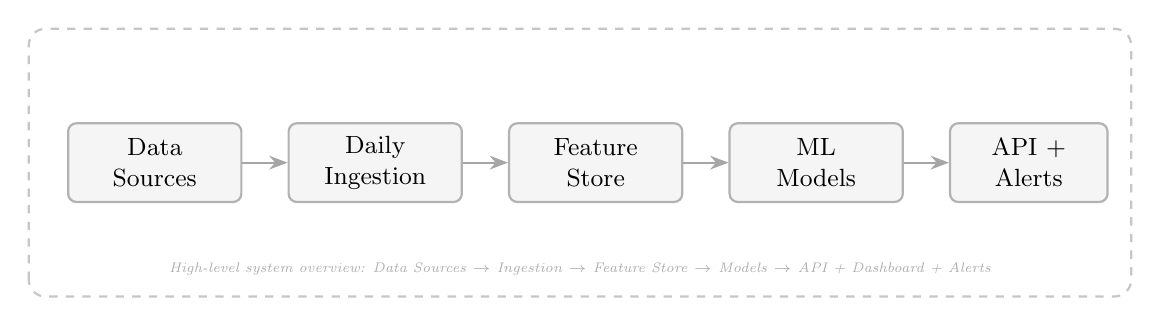
\begin{tikzpicture}[
  box/.style={rectangle, rounded corners=3pt, draw=gray!60, thick,
              fill=gray!8, font=\small, align=center, minimum height=1cm},
  arr/.style={->, >=Stealth, thick, gray!70}
]
  \draw[dashed, thick, gray!45, rounded corners=6pt] (-0.5,-0.7) rectangle (13.5,2.7);
  \node[gray!65, font=\tiny\itshape] at (6.5,-0.35)
        {High-level system overview: Data Sources $\to$ Ingestion $\to$ Feature Store $\to$ Models $\to$ API + Dashboard + Alerts};
  \node[box, minimum width=2.2cm] (src)  at (1.1,1)    {Data\\Sources};
  \node[box, minimum width=2.2cm] (ing)  at (3.9,1)    {Daily\\Ingestion};
  \node[box, minimum width=2.2cm] (feat) at (6.7,1)    {Feature\\Store};
  \node[box, minimum width=2.2cm] (mod)  at (9.5,1)    {ML\\Models};
  \node[box, minimum width=2.0cm] (out)  at (12.2,1)   {API +\\Alerts};
  \draw[arr] (src) -- (ing);
  \draw[arr] (ing) -- (feat);
  \draw[arr] (feat) -- (mod);
  \draw[arr] (mod) -- (out);
\end{tikzpicture}
\caption{High-level overview of the ChiangMai Air Quality Alert System (CAAS).}
\label{fig:system_overview}
\end{figure}

\section{Data Pipeline Design}

\subsection{Data Sources}

The pipeline integrates three data sources, each providing a distinct signal relevant to PM2.5 forecasting in Northern Thailand.

\begin{table}[H]
\centering
\caption{Summary of integrated data sources}
\label{tab:data_sources}
\begin{tabularx}{\textwidth}{@{}p{3cm}p{3cm}p{2cm}X@{}}
\toprule
\textbf{Source} & \textbf{Provider} & \textbf{Type} & \textbf{Coverage \& Granularity} \\
\midrule
PM2.5 concentration & air4thai / PCD Thailand & Excel + REST API & 2011--2025, stations 35T \& 36T, Chiang Mai (daily average) \\[4pt]
Historical weather   & Open-Meteo API          & REST API         & Chiang Mai coordinates (daily) \\[4pt]
Fire hotspots        & NASA FIRMS API          & REST API         & Northern Thailand bounding box (daily) \\
\bottomrule
\end{tabularx}
\end{table}

The primary station is 35T (Chiang Mai City Hall, Chang Phueak), with station 36T (Yupparaj School, Si Phum) serving as a fallback during gaps. The two stations exhibit a Pearson correlation of $r = 0.94$, confirming 36T as a reliable substitute for short-duration absences at the primary station. The full training dataset comprises approximately 5,475 daily observations spanning 15 years.

\subsection{Ingestion Method}

Data ingestion follows a two-mode strategy. A one-time historical load parses all 15 PCD Excel files (one per year, 2011--2025) to build the initial training corpus. Ongoing ingestion runs daily at 06:00 local time via a scheduled GitHub Actions workflow, retrieving the previous day's data from all three sources before executing the forecast pipeline.

Batch ingestion (rather than streaming) is appropriate for this use case because daily forecast granularity provides no operational benefit from sub-hourly data updates.

\subsection{Transformation Pipeline}

Transformations are applied in the following order within each pipeline execution:

\begin{enumerate}
  \item \textbf{Schema validation} --- verify expected columns, data types, and valid date range; pipeline halts immediately on any violation with no silent failures.
  \item \textbf{Missing value handling} --- interpolate PM2.5 gaps of up to three consecutive days using lag and rolling mean; substitute 36T station data for longer gaps; set fire count to zero on days with no detected hotspots.
  \item \textbf{Unit normalisation} --- standardise column names, numeric types, and date formats across all three source schemas.
  \item \textbf{Feature engineering} --- compute all derived features as described in Section~3.3.
  \item \textbf{Target variable creation} --- generate PM2.5 forward-shifted targets for $t+1$, $t+3$, and $t+7$.
\end{enumerate}

Orchestration is managed by GitHub Actions (cron: \texttt{0 6 * * *}). Each step logs success or failure explicitly, and checkpoints are saved after each step to enable pipeline resumption without re-running from scratch.

\section{Feature Engineering}

The full feature set comprises 44 engineered features organised into two groups: temporal autocorrelation features and contextual environmental features.

\subsection{Temporal Features}

\begin{table}[H]
\centering
\caption{Temporal autocorrelation and calendar features}
\label{tab:temporal_features}
\begin{tabularx}{\textwidth}{@{}lX@{}}
\toprule
\textbf{Feature} & \textbf{Description} \\
\midrule
\texttt{PM25\_lag1/2/3/7/14}       & PM2.5 values 1--14~days prior; captures short-term autocorrelation \\
\texttt{PM25\_roll3/7/14/30\_mean} & Rolling mean over 3--30~day windows; captures medium-term trend \\
\texttt{PM25\_roll7/30\_std}       & Rolling standard deviation; quantifies pollution volatility \\
\texttt{month\_sin}, \texttt{month\_cos} & Cyclical month encoding; avoids ordinality assumption \\
\texttt{day\_sin}, \texttt{day\_cos}     & Cyclical day-of-year encoding \\
\texttt{is\_haze\_season}          & Binary: 1 if January--April \\
\texttt{is\_rainy\_season}         & Binary: 1 if May--October \\
\texttt{is\_cool\_season}          & Binary: 1 if November--December \\
\bottomrule
\end{tabularx}
\end{table}

\subsection{Contextual Environmental Features}

\begin{table}[H]
\centering
\caption{Contextual meteorological and fire activity features}
\label{tab:contextual_features}
\begin{tabularx}{\textwidth}{@{}lX@{}}
\toprule
\textbf{Feature} & \textbf{Description} \\
\midrule
\texttt{north\_avg\_PM25}       & Average PM2.5 across 15 Northern Thailand stations; regional smoke signal \\
\texttt{north\_max\_PM25}       & Maximum PM2.5 across Northern Thailand stations \\
\texttt{wind\_speed}, \texttt{wind\_dir} & Wind speed and direction from Open-Meteo; governs smoke transport \\
\texttt{humidity}, \texttt{temperature} & Atmospheric conditions from Open-Meteo \\
\texttt{boundary\_layer\_height}        & Atmospheric mixing height; key driver of surface PM2.5 accumulation \\
\texttt{fire\_count}             & Daily hotspot count within 100~km of Chiang Mai (NASA FIRMS) \\
\texttt{fire\_frp\_sum}          & Total Fire Radiative Power; proxy for fire intensity and smoke volume \\
\bottomrule
\end{tabularx}
\end{table}

\subsection{Target Variables}

\begin{table}[H]
\centering
\caption{Target variables for regression and classification tasks}
\label{tab:targets}
\begin{tabular}{@{}llp{7cm}@{}}
\toprule
\textbf{Variable}    & \textbf{Type}              & \textbf{Definition} \\
\midrule
\texttt{PM25\_next1} & Regression                 & PM2.5 concentration tomorrow (\textmu g/m\textsuperscript{3}) \\
\texttt{PM25\_next3} & Regression                 & PM2.5 concentration in 3~days \\
\texttt{PM25\_next7} & Regression                 & PM2.5 concentration in 7~days \\
\texttt{alert\_next1}& Binary classification      & 1 if PM2.5 tomorrow $>$ 50~\textmu g/m\textsuperscript{3} \\
\texttt{alert\_next3}& Binary classification      & 1 if PM2.5 in 3~days $>$ 50~\textmu g/m\textsuperscript{3} \\
\bottomrule
\end{tabular}
\end{table}

\section{Model Training and Evaluation}

\subsection{Model Selection Rationale}

This project employs a two-model comparative strategy rather than assuming \textit{a priori} that one architecture will outperform the other. This decision is motivated by an important consideration raised during proposal review: with approximately 5,475 daily observations, does a sequential deep learning model offer genuine advantages over a well-tuned gradient boosting model with rich temporal features?

The honest answer is: not necessarily. The comparative experimental design allows the data to answer this question empirically.

\subsubsection{XGBoost --- Primary Baseline Model}

XGBoost~\cite{chen2016xgboost} is the primary baseline and a strong candidate for the production model. Its key advantages for this dataset include:
\begin{itemize}
  \item Efficient and robust training on moderate-sized tabular data with limited overfitting risk.
  \item Native handling of missing values without imputation.
  \item Strong regularisation (L1/L2) to prevent overfitting on the approximately 5,475-sample training set.
  \item Interpretability via SHAP feature importance analysis, enabling model behaviour explanation to non-technical stakeholders.
  \item Given that the temporal features already encode autocorrelation and rolling patterns explicitly, XGBoost operates on a feature representation that has effectively ``pre-digested'' the sequence structure into a flat tabular form---which is precisely where gradient boosting excels.
\end{itemize}

\subsubsection{LSTM --- Comparative Sequential Model}

An LSTM network~\cite{hochreiter1997lstm} with a 30-day input window is deployed as a comparative sequential model. The rationale for including LSTM is not an expectation of across-the-board superiority, but a specific testable hypothesis:

\textbf{Hypothesis:} XGBoost is expected to perform strongly on t+1 forecasting, where the lag-1 feature is highly predictive and the fixed-window feature representation is adequate. LSTM may demonstrate advantages on longer-horizon forecasts (t+3, t+7), where multi-step sequential dependencies and the compounding of seasonal atmospheric signals may be better captured through explicit sequence modelling than through the static lag features available to XGBoost.

Regarding the sample size: while the dataset contains approximately 5,475 row-level observations, training an LSTM with a 30-day sliding window generates approximately 5,400 overlapping sequence samples of length 30. Regularisation measures including dropout (rate 0.2--0.3), L2 weight decay, and early stopping will be applied to mitigate overfitting risk. If LSTM training proves unstable or overfitting cannot be controlled, the XGBoost model will serve as the sole production model---a fully acceptable outcome since the comparative evaluation is itself the contribution.

\subsection{Chronological Data Split}

A strict chronological split is used with no data shuffling, respecting the temporal dependency structure and simulating realistic deployment conditions.

\begin{table}[H]
\centering
\caption{Chronological training, validation, and test split}
\label{tab:data_split}
\begin{tabular}{@{}llp{8.5cm}@{}}
\toprule
\textbf{Split} & \textbf{Period} & \textbf{Rationale} \\
\midrule
Training   & 2011--2022 & 12 years; includes multiple complete haze seasons \\
Validation & 2023       & Hyperparameter tuning; one complete annual cycle \\
Test       & 2024--2025 & Fully unseen; includes the most recent haze seasons \\
\bottomrule
\end{tabular}
\end{table}

% ============================================================
%  CHAPTER 4 — SYSTEM ARCHITECTURE
% ============================================================
\chapter{SYSTEM ARCHITECTURE AND PIPELINE DESIGN}

\section{Architecture Overview}

The CAAS architecture follows a layered design with clearly separated concerns across ingestion, storage, compute, serving, and monitoring layers. All components are deployed on AWS using the available Learner Lab credits.

\begin{figure}[H]
\centering
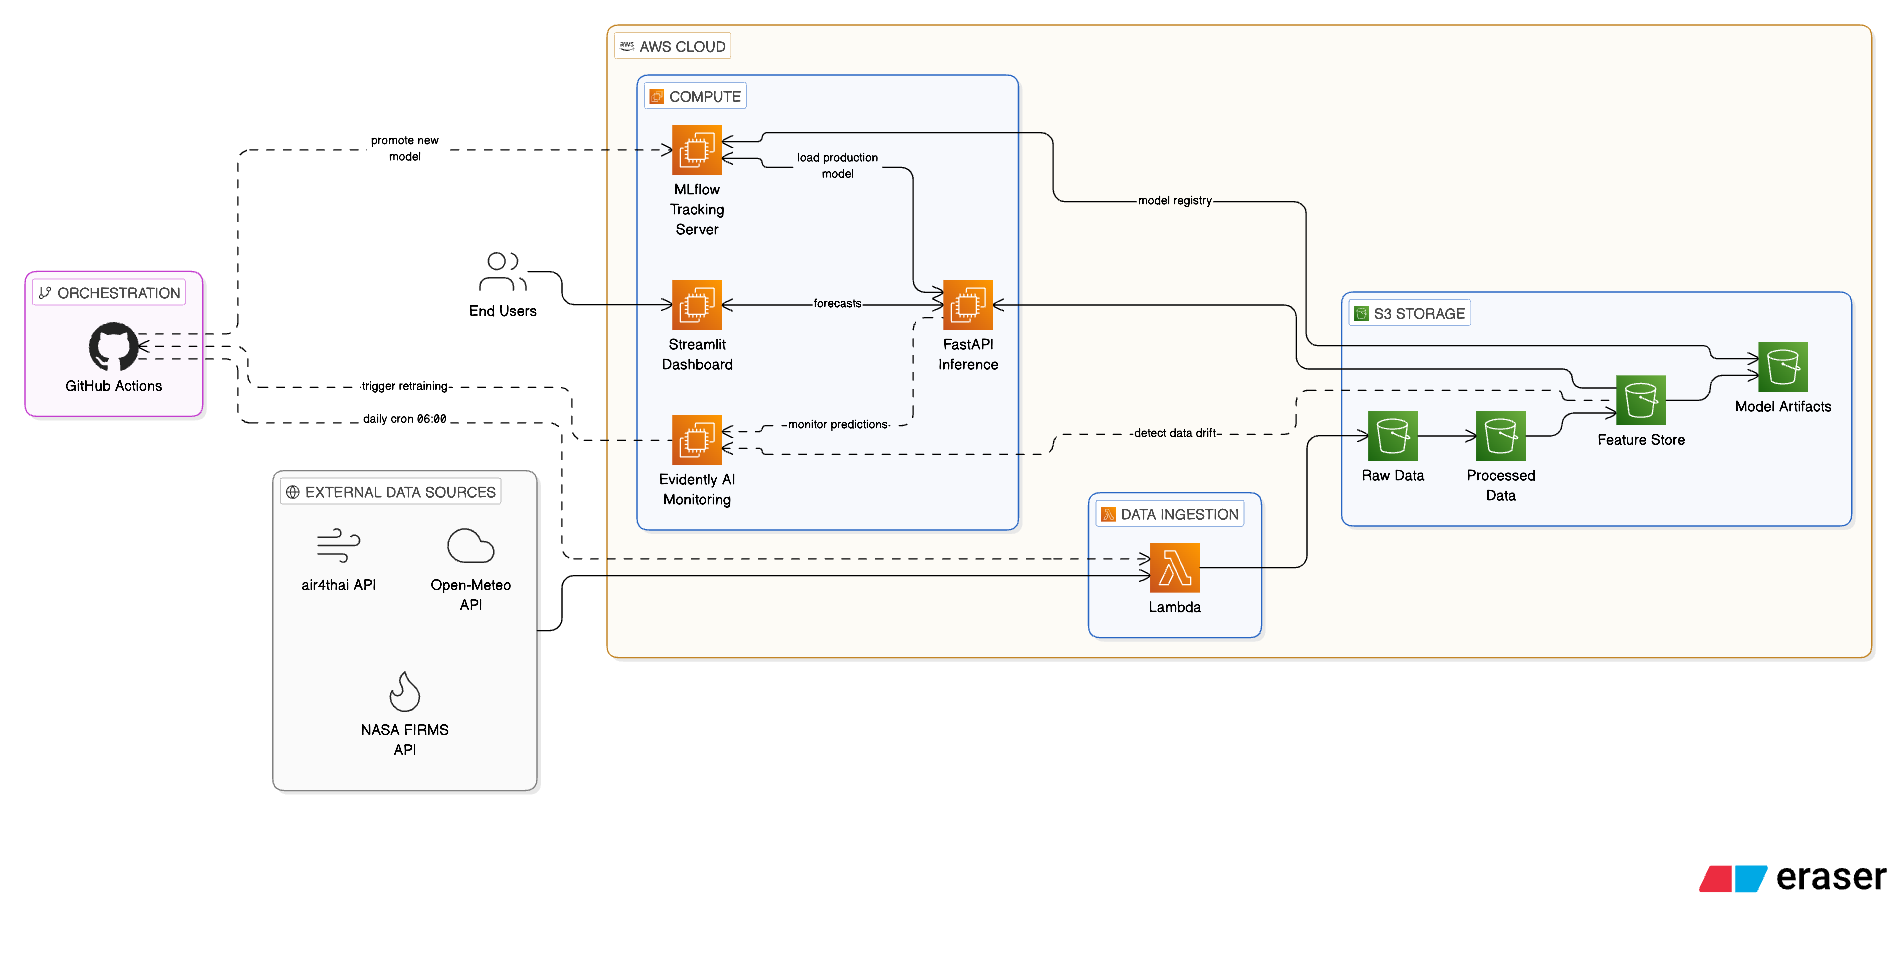
\includegraphics[width=\textwidth]{fig_cloud_architecture.png}
\caption{AWS cloud architecture for the ChiangMai Air Quality Alert System (CAAS). The pipeline spans three external data sources (air4thai API, Open-Meteo API, NASA FIRMS API), an AWS Lambda ingestion layer triggered daily at 06:00 UTC+7 via GitHub Actions, four S3 storage tiers (Raw, Processed, Feature Store, Model Artifacts), and a compute layer comprising MLflow Tracking Server, FastAPI Inference Server, Streamlit Dashboard, and Evidently AI drift monitoring. Dashed arrows indicate orchestration triggers and automated retraining signals.}
\label{fig:aws_architecture}
\end{figure}

\section{Storage Layers}

The storage architecture separates data by processing stage into four layers on Amazon S3:

\begin{itemize}
  \item \textbf{Raw Layer} (\texttt{s3://caas/raw/pm25/}, \texttt{raw/weather/}, \texttt{raw/fire/}) --- Immutable, append-only source data exactly as ingested. Files are never overwritten.
  \item \textbf{Processed Layer} (\texttt{s3://caas/processed/merged/}) --- Cleaned, validated, and schema-enforced daily merged files.
  \item \textbf{Feature Store} (\texttt{s3://caas/features/pm25\_daily\_chiangmai.csv}) --- ML-ready dataset with all 44 features and target columns, versioned by run date.
  \item \textbf{Model Artifacts} --- MLflow artifact store containing trained model files, hyperparameters, evaluation metrics, SHAP plots, confusion matrices, and loss curves per experiment run.
\end{itemize}

\section{MLOps Lifecycle}

\subsection{Experiment Tracking}

All training runs are logged to MLflow, recording: hyperparameters (learning rate, \texttt{n\_estimators}, LSTM units, sequence length, dropout rate), evaluation metrics (RMSE, MAE, $R^2$, Precision, Recall, F1, AUROC), artifacts (model file, feature importance plot, confusion matrix, loss curves), and the dataset version (snapshot date) used for training. This enables full reproducibility and direct side-by-side comparison between XGBoost and LSTM runs.

\subsection{Model Versioning and Promotion}

Models are managed through the MLflow Model Registry using a three-stage promotion workflow:
\[
\text{[Staging]} \;\longrightarrow\; \text{[Validation]} \;\longrightarrow\; \text{[Production]}
\]

\begin{itemize}
  \item \textbf{Staging} --- Newly trained model awaiting metric evaluation.
  \item \textbf{Validation} --- Model has passed RMSE and Recall thresholds; ready for deployment review.
  \item \textbf{Production} --- Currently serving model; only one model occupies this stage at any time.
\end{itemize}

Promotion to Production is automated when metrics pass predefined thresholds. Previous Production models are archived, not deleted, to enable rollback.

\begin{figure}[H]
\centering
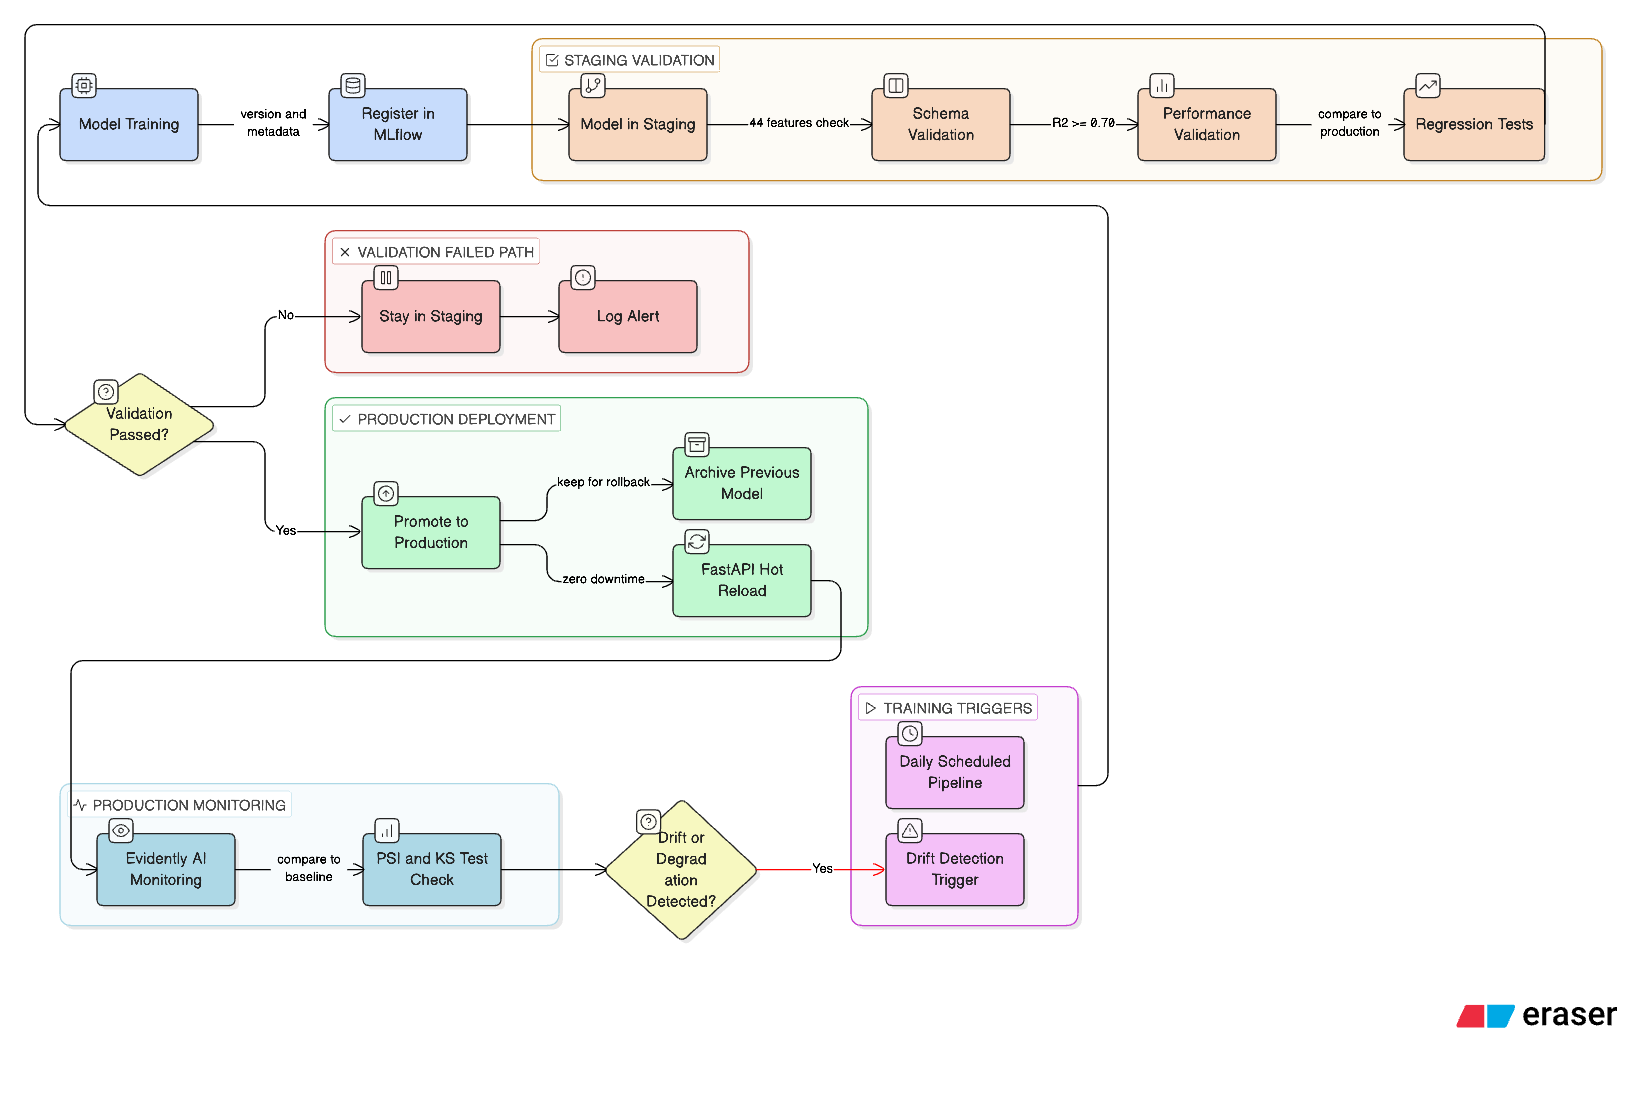
\includegraphics[width=\textwidth]{fig_model_promotion.png}
\caption{MLflow model promotion and lifecycle flow. Newly trained models are registered in MLflow and enter the Staging stage, where they undergo schema validation (44-feature check), performance validation ($R^2 \geq 0.70$), and regression tests against the current Production model. Failed validation keeps the model in Staging with an alert logged. On success, the model is promoted to Production with zero-downtime FastAPI hot-reload; the previous Production model is archived for rollback. Evidently AI drift detection and a daily scheduled pipeline serve as the primary retraining triggers.}
\label{fig:model_promotion}
\end{figure}

\subsection{GitHub Actions CI/CD Retraining Pipeline}

Proposal review raised the specific question of what stages exist in the GitHub Actions retraining workflow, which step blocks promotion, and whether there are charges. This subsection provides complete answers.

The retraining workflow (\texttt{.github/workflows/retrain.yml}) is triggered by three events: a cron schedule (December 1 annually), a webhook from the drift monitor when any threshold in Table~\ref{tab:drift_triggers} is exceeded, or a manual \texttt{workflow\_dispatch} call. The pipeline comprises six sequential stages:

\begin{table}[H]
\centering
\caption{GitHub Actions retraining pipeline stages}
\label{tab:github_stages}
\begin{tabularx}{\textwidth}{@{}p{0.4cm}p{4.0cm}X@{}}
\toprule
\textbf{\#} & \textbf{Stage} & \textbf{Description and failure behaviour} \\
\midrule
1 & \texttt{data-snapshot}   & Pull latest PM2.5, weather, and FIRMS data; validate schema; save versioned snapshot to S3. \textit{Failure: halt pipeline, send alert, no model update.} \\[4pt]
2 & \texttt{feature-build}   & Run \texttt{build\_features.py}; produce updated \texttt{features.csv}. \textit{Failure: halt.} \\[4pt]
3 & \texttt{model-train}     & Train XGBoost and LSTM candidate models on updated data. Log all runs to MLflow. \textit{Failure: halt.} \\[4pt]
4 & \textbf{\texttt{validation-gate}} & \textbf{Blocking stage.} Compare candidate vs.\ champion on 90-day rolling window. Must satisfy: (a) MAE improvement $\geq 5\%$; (b) alert F1 $\geq 0.75$; (c) 45-feature schema match. \textit{Failure: candidate stays in Staging; champion unchanged; failure reason logged.} \\[4pt]
5 & \texttt{mlflow-register} & Tag validated candidate as \texttt{Production}; archive previous champion as \texttt{Archived}. \\[4pt]
6 & \texttt{deploy}          & Pull new \texttt{Production} model to EC2; zero-downtime FastAPI hot-reload via uvicorn \texttt{--reload}. \\
\bottomrule
\end{tabularx}
\end{table}

\textbf{Regarding cost:} The project repository is public on GitHub. Public repositories receive unlimited GitHub Actions minutes at no charge. For a private repository, the free tier provides 2,000 minutes per month; a typical full retraining run (data pull + feature build + XGBoost + LSTM + validation) is estimated at 30--50 minutes. At a maximum of 4 triggered retraining runs per month during the haze season, this totals approximately 160--200 minutes---comfortably within the free tier, resulting in \textbf{\$0 additional cost} for CI/CD.

\subsection{Deployment Strategy}

The deployment architecture uses a hybrid batch and real-time API approach. The primary daily pipeline runs at 06:00 via GitHub Actions: it ingests the previous day's data, generates t+1/3/7 forecasts, and stores results to S3. A FastAPI service exposes \texttt{/predict} and \texttt{/alert} endpoints for the Streamlit dashboard and external consumers.

\begin{figure}[H]
\centering
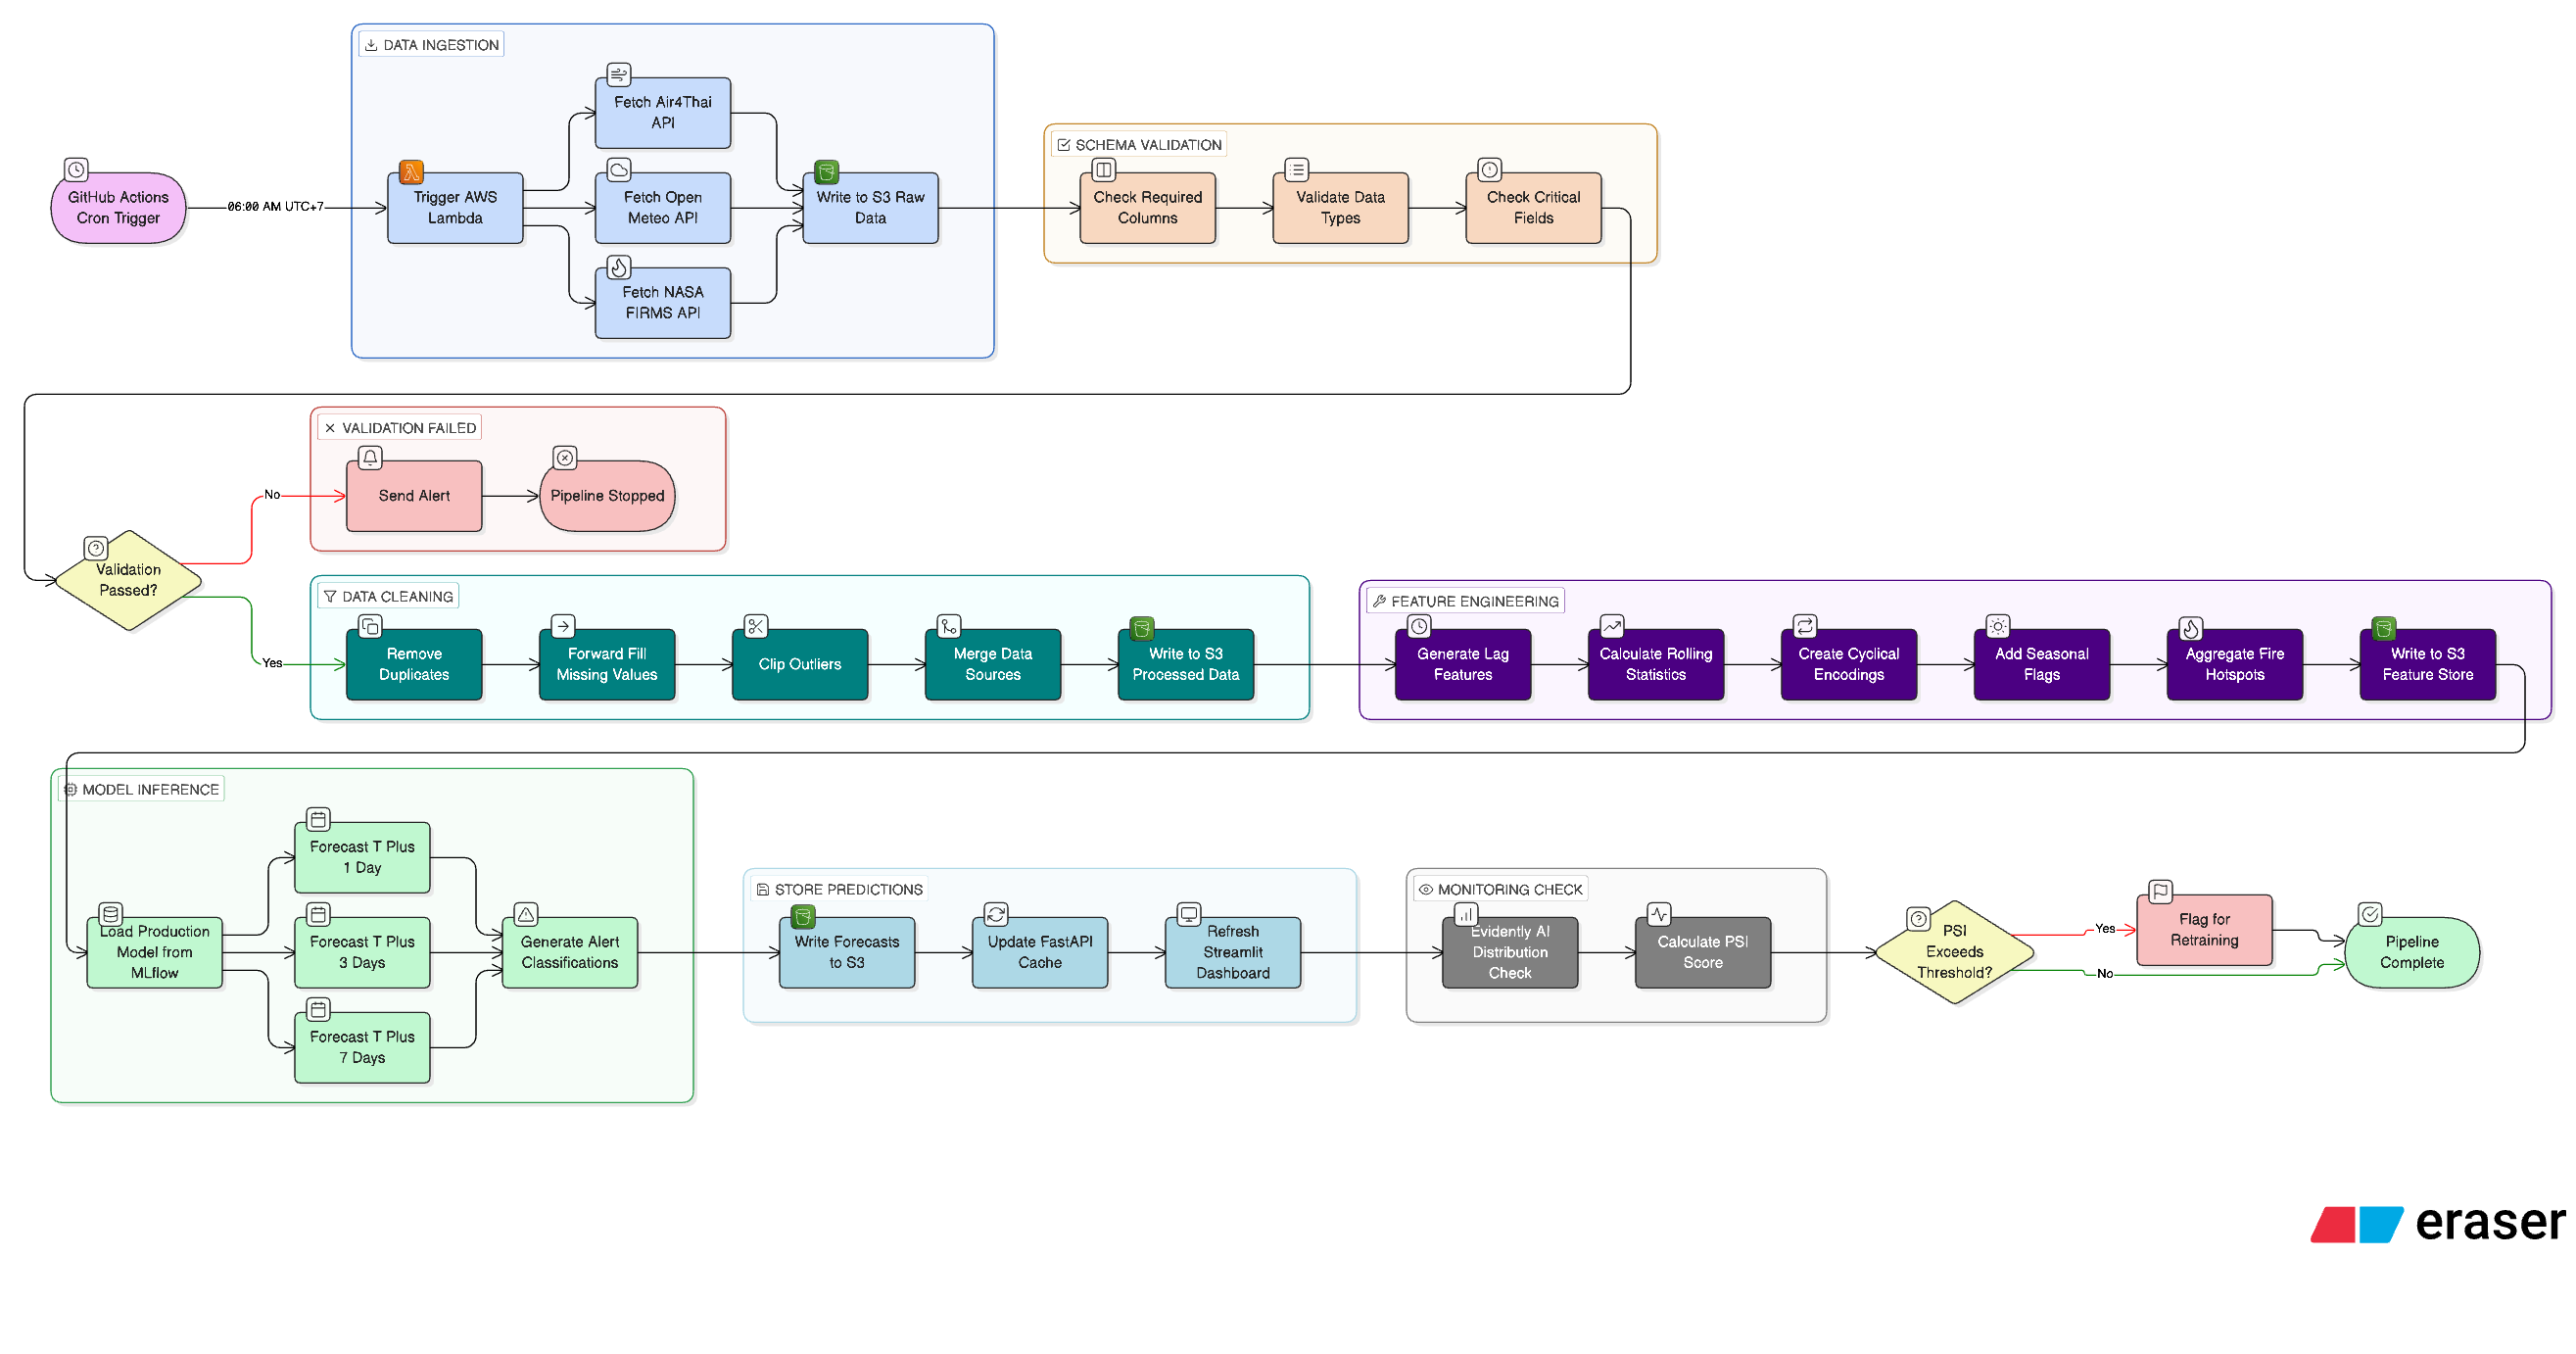
\includegraphics[width=\textwidth]{fig_daily_pipeline.png}
\caption{Daily MLOps pipeline execution flow triggered at 06:00~UTC+7 via GitHub Actions. The pipeline comprises seven stages: (1)~Data Ingestion via AWS Lambda fetching from air4thai, Open-Meteo, and NASA FIRMS APIs into S3 Raw; (2)~Schema Validation with a failure branch that sends an alert and stops the pipeline; (3)~Data Cleaning including duplicate removal, forward-fill for missing values, and outlier clipping; (4)~Feature Engineering producing 44 features (lag, rolling statistics, cyclical encodings, seasonal flags, fire hotspots) stored to S3 Feature Store; (5)~Model Inference generating PM2.5 regression values and alert-level classifications for t+1, t+3, and t+7 horizons; (6)~Store Predictions to S3 and update the FastAPI cache; (7)~Monitoring Check using Evidently AI PSI drift detection, flagging for retraining if PSI~$>$~0.2.}
\label{fig:pipeline_flow}
\end{figure}

\begin{figure}[H]
\centering
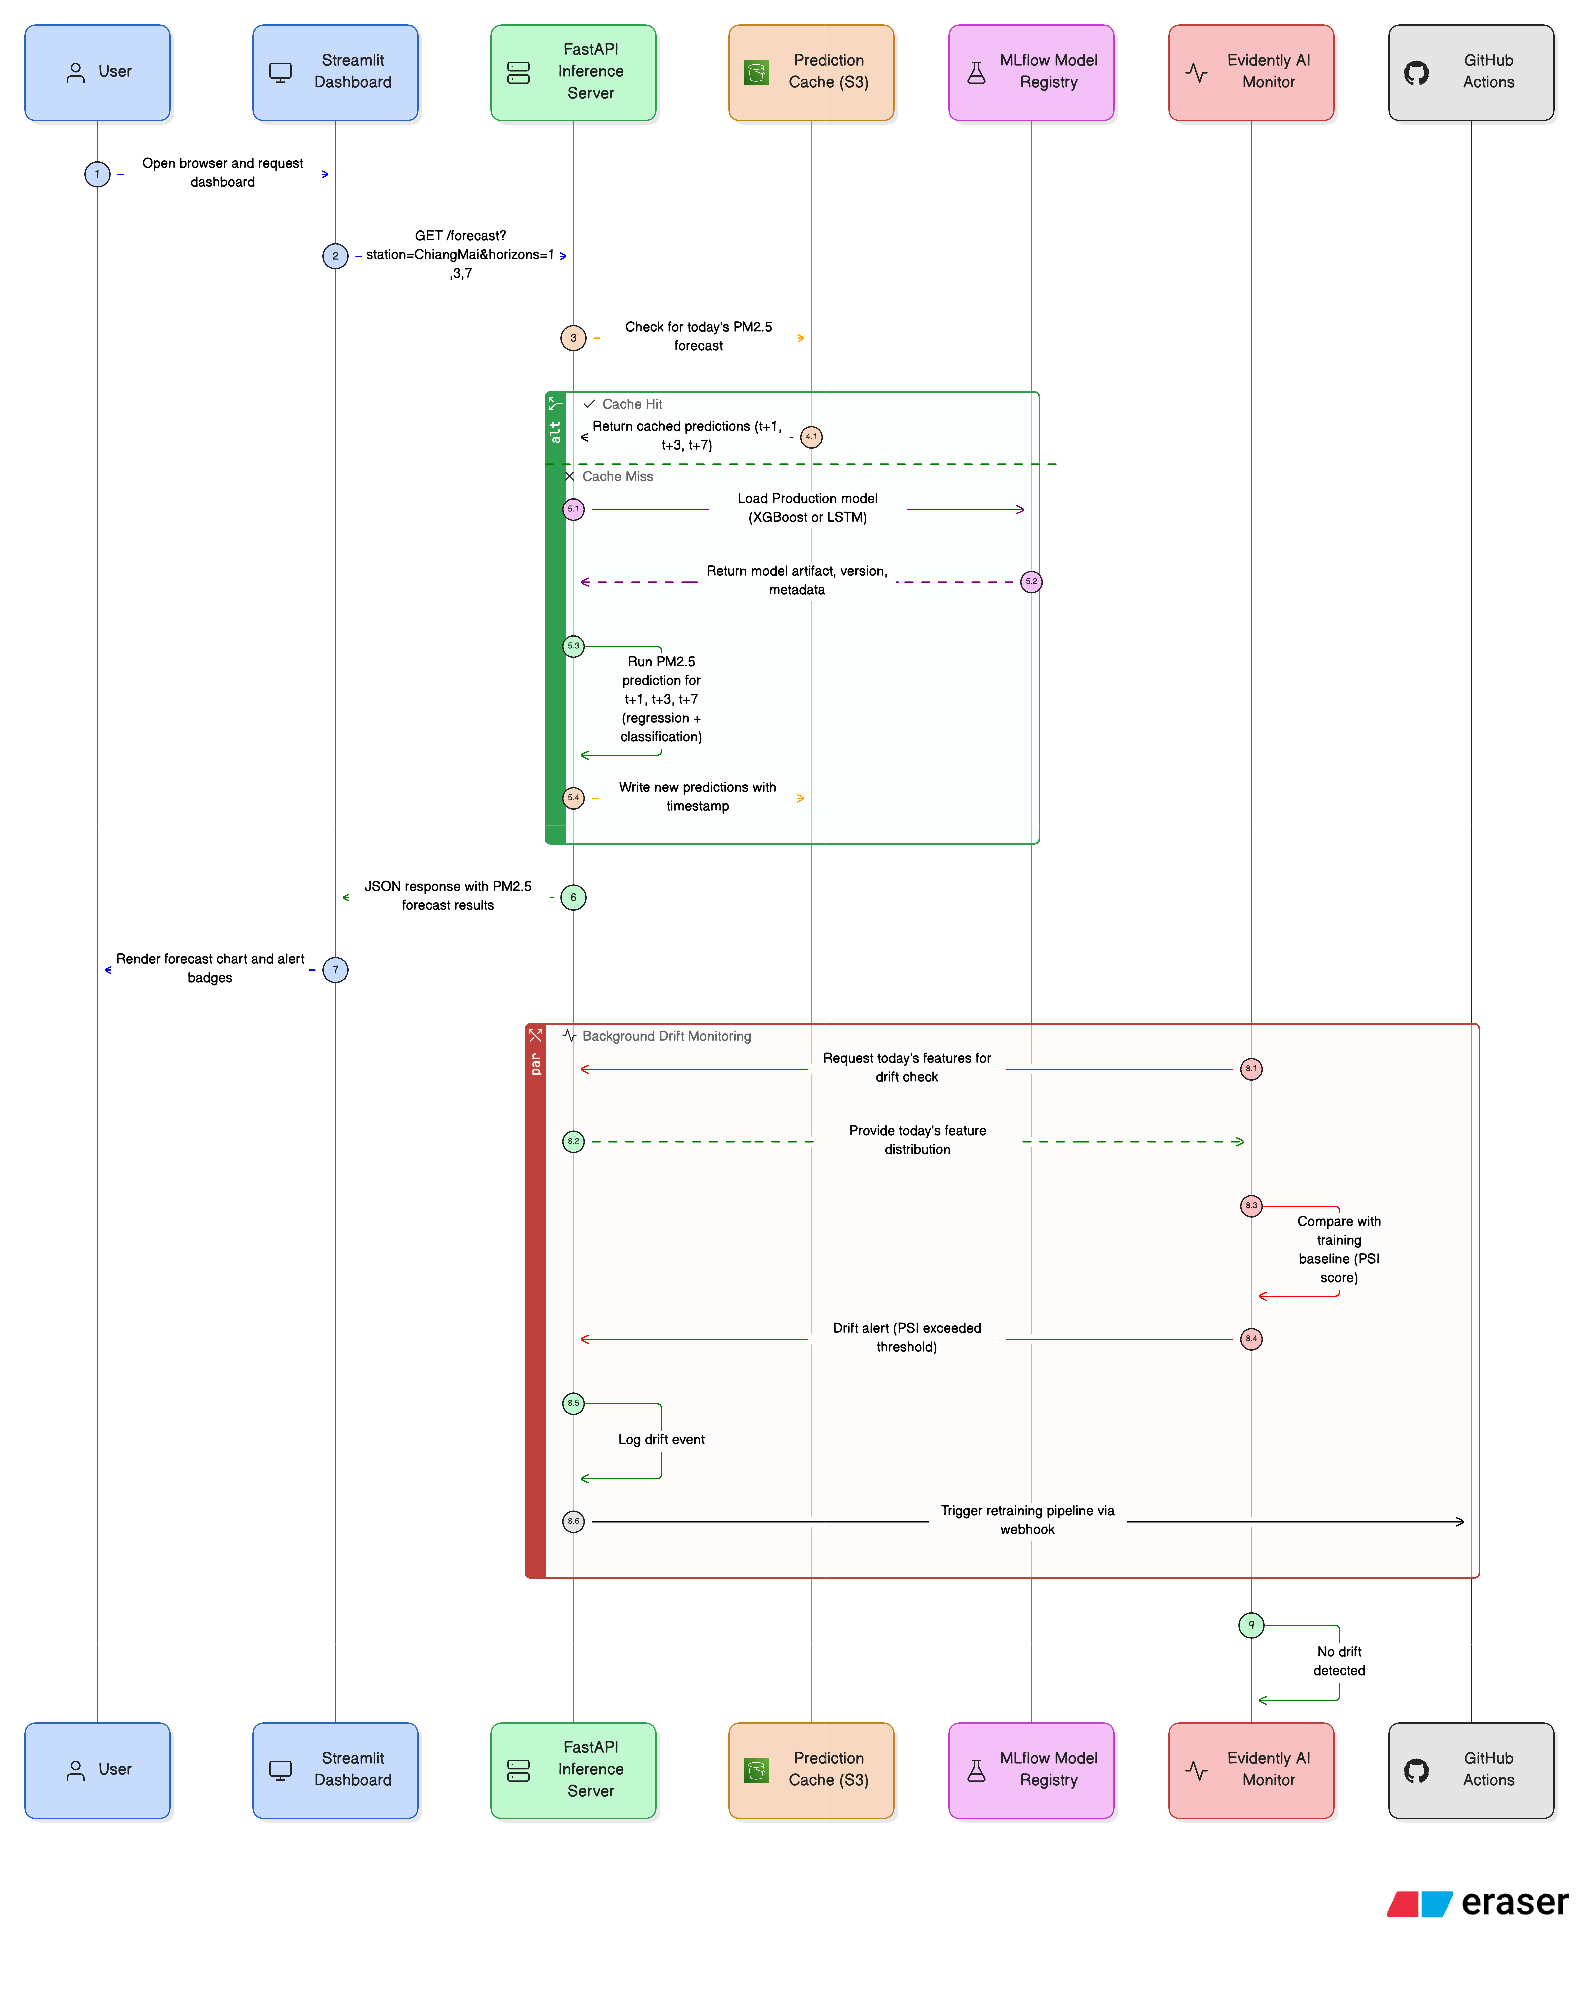
\includegraphics[width=0.85\textwidth]{fig_sequence_flow.png}
\caption[End-to-end PM2.5 forecast request flow for the CAAS system.]{End-to-end PM2.5 forecast request flow for the CAAS system. When a user opens the Streamlit Dashboard, it sends a \texttt{GET /forecast?station=ChiangMai\&horizons=1,3,7} request to the FastAPI Inference Server. The server first queries the S3 Prediction Cache: on a cache hit, predictions for t+1, t+3, and t+7 days are returned immediately; on a cache miss, the server loads the Production model from MLflow, runs PM2.5 regression and alert-level classification inference, writes the results to the cache, and returns a JSON response. In parallel, Evidently AI performs background drift monitoring by comparing today's feature distribution against the training baseline using PSI scoring. If PSI exceeds 0.2, a drift alert triggers the GitHub Actions retraining pipeline via webhook.}
\label{fig:sequence_flow}
\end{figure}

\section{Monitoring and Automated Retraining}

This section provides a unified definition of drift detection and retraining logic, addressing feedback received during the proposal review that noted inconsistency between drift signals, thresholds, and retraining triggers.

\subsection{Drift Detection Signals}

Three independent drift signals are monitored, each targeting a distinct failure mode:

\begin{table}[H]
\centering
\caption{Unified drift detection signals, thresholds, and actions}
\label{tab:drift_triggers}
\begin{tabularx}{\textwidth}{@{}p{2.8cm}p{2.2cm}p{2.5cm}X@{}}
\toprule
\textbf{Signal} & \textbf{Tool} & \textbf{Threshold} & \textbf{Action} \\
\midrule
7-day rolling MAE on live predictions & MLflow + daily pipeline & ${>}$15~\textmu g/m\textsuperscript{3} (t+1) & Flag for retraining candidate; alert logged \\[6pt]
Feature distribution drift (PSI) on \texttt{pm25\_lag1}, \texttt{wind\_speed}, \texttt{hotspot\_50km} & Evidently AI (weekly) & PSI~${>}$~0.2 & Flag data drift; inspect source data quality \\[6pt]
Kolmogorov-Smirnov test on 30-day residual distribution & Evidently AI (monthly) & $p < 0.05$ & Flag concept drift; trigger retraining \\[6pt]
Scheduled (annual) & GitHub Actions (cron) & December 1 each year & Forced retrain incorporating latest full year \\
\bottomrule
\end{tabularx}
\end{table}

\subsection{Retraining Validation Gate}

Retraining is triggered when \textit{any} signal in Table~\ref{tab:drift_triggers} fires. However, a new model is not automatically promoted to production. The following gate must be passed before promotion:

\begin{enumerate}
  \item \textbf{Schema validation}: candidate model accepts exactly the same 45-feature input schema.
  \item \textbf{Performance gate}: candidate model must achieve MAE improvement of at least 5\% over the current production champion on a 90-day rolling validation window.
  \item \textbf{Alert recall gate}: candidate alert F1-score (threshold~$>$~50~\textmu g/m\textsuperscript{3}) must be $\geq$~0.75 on the validation window.
\end{enumerate}

If the candidate fails any gate, it remains in MLflow \texttt{Staging} status and the champion continues to serve predictions. The pipeline logs the failure reason explicitly and raises a notification. This design ensures that automated retraining never silently degrades production accuracy.

\subsection{Evidently AI Monitoring Configuration}

Evidently AI runs as a \textbf{scheduled weekly report} (GitHub Actions cron), not as an always-on daemon. This eliminates the idle compute cost while still providing regular drift visibility. Reports are stored as HTML artifacts in S3 and linked from the Streamlit dashboard. Only when a report flags a threshold breach is any human or automated action triggered.

\section{Infrastructure and Cost Estimate}

Proposal review feedback noted inconsistency between the stated total cost and the individual component breakdown, and questioned whether always-on serving components (FastAPI, Streamlit, MLflow) are compatible with a low monthly budget. This section provides an accurate reconciliation.

\textbf{Key architectural decision}: FastAPI, Streamlit, and the MLflow Tracking Server all run on a \textit{single shared} EC2~t3.micro instance. There is no separate instance per service. Evidently AI runs as a scheduled weekly batch job, not as an always-on process. This co-location is feasible because these services are lightweight and rarely active simultaneously under the expected load of one automated daily pipeline run and occasional human dashboard access.

\begin{table}[H]
\centering
\caption{Revised monthly AWS infrastructure cost breakdown}
\label{tab:cost_revised}
\begin{tabularx}{\textwidth}{@{}p{3.2cm}Xp{3.8cm}@{}}
\toprule
\textbf{Service} & \textbf{Usage detail} & \textbf{Monthly cost} \\
\midrule
EC2 t3.micro (shared) & FastAPI + Streamlit + MLflow UI, always-on; $\sim$\$0.0104/hr & \$7.50 (on-demand) / \$0 (Learner Lab) \\[4pt]
Amazon S3             & $\sim$5~GB total (raw + processed + features + models + reports) & \$0.12 \\[4pt]
AWS Lambda            & Ingestion trigger: 1 invocation/day $\times$ 5~min $\times$ 128~MB & \$0.00 (well within free tier) \\[4pt]
GitHub Actions        & Orchestration: public repo = unlimited; private = $\sim$160~min/month (retraining) $\ll$ 2,000 free tier & \$0.00 \\[4pt]
Open-Meteo API        & Free academic archive endpoint                        & \$0.00 \\[4pt]
NASA FIRMS API        & Free with registered MAP key                          & \$0.00 \\[4pt]
\midrule
\textbf{Total}        & All services combined                                 & \textbf{\$7.62 -- \$8/month} \\
\textbf{(Learner Lab)}& EC2 covered by credits                                & \textbf{\$0.12/month} \\
\bottomrule
\end{tabularx}
\end{table}

The corrected total is \textbf{\$8/month} under standard AWS pricing, or effectively \textbf{under \$1/month} within the AWS Learner Lab environment. This replaces the previously stated \$2--8 range, which was inconsistent with the EC2 cost alone exceeding the lower bound.

\section{Data Quality Management}

Data quality is treated as a first-class concern in the pipeline. Each ingested record must pass schema validation before entering the processing layer; any violation halts the pipeline immediately with an explicit error log and GitHub Actions email notification. Silent failures are not permitted.

\subsection{Missing Value Handling Strategy}

\begin{table}[H]
\centering
\caption{Missing value handling by data source}
\label{tab:missing_values}
\begin{tabularx}{\textwidth}{@{}p{3cm}p{3.5cm}X@{}}
\toprule
\textbf{Source} & \textbf{Expected Missing Rate} & \textbf{Handling Strategy} \\
\midrule
air4thai PM2.5 (35T) &
  $\sim$2--3\% per year &
  Gaps $\leq$3 consecutive days: linear interpolation using adjacent lag and rolling mean values. Gaps $>$3 days: substitute 36T station data ($r = 0.94$). All imputed rows flagged with \texttt{is\_imputed = 1} column. \\[6pt]
Open-Meteo weather &
  Near zero (reanalysis data) &
  No action required; reanalysis fills missing observations by design. \\[6pt]
NASA FIRMS fire &
  Zero hotspots on some days is valid (not missing) &
  Fill \texttt{fire\_count = 0} and \texttt{fire\_frp\_sum = 0} on days with no detected hotspots in the bounding box. \\
\bottomrule
\end{tabularx}
\end{table}

\subsection{Schema Validation Rules}

Every pipeline run enforces the following validation checks before processing proceeds:
\begin{itemize}
  \item Expected column names and data types are present and correct.
  \item Date range is within bounds and contains no duplicate dates.
  \item Numeric values fall within physically plausible ranges (e.g., PM2.5 $\in [0, 500]$~\textmu g/m\textsuperscript{3}).
  \item Station identifiers match expected codes (35T, 36T).
\end{itemize}
Earlier PCD files (2011--2017) may differ in column count due to network expansion; the validator applies source-year-specific schemas to handle this gracefully.

\subsection{Pipeline Health Monitoring}

Each pipeline step (ingest $\to$ validate $\to$ preprocess $\to$ feature engineering $\to$ predict) emits structured logs containing: step name, timestamp, input row count, output row count, and pass/fail status. If any step fails, all downstream steps are blocked immediately. A data freshness check after each ingestion run verifies that the latest PM2.5 record date matches yesterday; if data is more than two days stale, the source is flagged as potentially unavailable and an alert is raised.

% ============================================================
%  CHAPTER 5 — EXPERIMENTAL PLAN AND EXPECTED CONTRIBUTIONS
% ============================================================
\chapter{EXPERIMENTAL PLAN AND EXPECTED CONTRIBUTIONS}

\section{Dataset Characteristics}

The training dataset comprises approximately 5,475 daily observations from 2011 to 2025, representing 15 complete annual cycles. Key statistical characteristics include:

\begin{itemize}
  \item \textbf{March 2025 average}: 55.1~\textmu g/m\textsuperscript{3} --- more than $3\times$ the WHO 24-hour guideline.
  \item \textbf{Single-day maximum}: 92.3~\textmu g/m\textsuperscript{3} (March 23, 2025).
  \item \textbf{Days exceeding Thailand's 25~\textmu g/m\textsuperscript{3} threshold}: 109 days (31\% of the year).
  \item \textbf{PM2.5 missing rate}: approximately 2--3\% per year.
  \item \textbf{Cross-station correlation} (35T vs.\ 36T): $r = 0.940$.
\end{itemize}

\section{Baseline Methods for Comparison}

Three strategies will be compared:

\begin{enumerate}
  \item \textbf{Persistence baseline} --- the forecast equals the most recent observed PM2.5 value (lag-1). This naive baseline establishes the lower bound that any model must exceed.
  \item \textbf{XGBoost with 44 engineered features} --- the primary tabular baseline described in Chapter~3.
  \item \textbf{LSTM with 30-day sequence window} --- the comparative sequential model.
\end{enumerate}

\section{Evaluation Metrics}

\begin{table}[H]
\centering
\caption{Evaluation metrics by task type and priority}
\label{tab:eval_metrics}
\begin{tabularx}{\textwidth}{@{}llX@{}}
\toprule
\textbf{Task} & \textbf{Metrics} & \textbf{Priority and Rationale} \\
\midrule
Regression (PM2.5 \textmu g/m\textsuperscript{3}) &
  RMSE, MAE, $R^2$ &
  RMSE is the primary regression metric; $R^2 \geq 0.70$ is the target benchmark. \\[6pt]
Classification (alert/no alert) &
  Precision, Recall, F1, AUROC &
  Recall is the primary classification metric. A missed true alert (false negative) carries greater public health cost than a false alarm (false positive). \\
\bottomrule
\end{tabularx}
\end{table}

\section{Experimental Setup}

Experiments will be conducted as follows:

\begin{enumerate}
  \item Both models trained on the 2011--2022 training set; hyperparameters tuned on the 2023 validation set using random search.
  \item Final evaluation on the 2024--2025 test set (fully unseen data).
  \item Separate experiments for each forecast horizon (t+1, t+3, t+7) to test whether any LSTM advantage is horizon-dependent.
  \item XGBoost SHAP analysis conducted to identify the most influential features for interpretability and domain insight.
  \item All runs logged to MLflow with full hyperparameter, metric, and artifact records for reproducibility.
\end{enumerate}

\section{Expected Contributions}

Following proposal review feedback, this section accurately frames the project's contribution. CAAS is not primarily a novel forecasting methodology---the models employed (XGBoost, LSTM) are established techniques. The contribution lies in the \textbf{production-grade integration} of multiple components into a coherent, automated, and self-maintaining operational system. This is precisely what the MLOps course is designed to develop and evaluate.

\begin{enumerate}
  \item \textbf{A production-ready MLOps reference pipeline} for environmental forecasting, demonstrating the complete operational lifecycle: multi-source ingestion $\to$ feature engineering $\to$ chronologically-split model training $\to$ MLflow experiment tracking $\to$ staged model promotion with validation gates $\to$ FastAPI serving $\to$ Streamlit public dashboard $\to$ automated drift detection and retraining. This end-to-end integration, applied to a genuine public-health problem, is the primary contribution.

  \item \textbf{An evidence-based model comparison} of XGBoost (tabular gradient boosting) versus LSTM (sequential deep learning) on 15 years of daily PM2.5 data, evaluated separately per forecast horizon (t+1, t+3, t+7). The production champion is selected empirically, not assumed in advance.

  \item \textbf{A reproducible 45-feature engineering framework} integrating PM2.5 autocorrelation, rolling statistics, cyclical calendar encodings, meteorological variables, and NASA FIRMS satellite fire hotspot signals into a unified ML-ready dataset.

  \item \textbf{A public health early-warning tool} providing Chiang Mai residents with 1-, 3-, and 7-day PM2.5 forecasts and automated hazardous-level alerts via a Streamlit dashboard.
\end{enumerate}

\section{Feasibility and Tool Selection}

All tools are open-source, well-documented, and either free or within Learner Lab credit limits. The technology stack is:

\begin{itemize}
  \item \textbf{Language}: Python 3.11
  \item \textbf{ML models}: XGBoost, TensorFlow/Keras (LSTM)
  \item \textbf{Experiment tracking}: MLflow
  \item \textbf{API serving}: FastAPI
  \item \textbf{Dashboard}: Streamlit
  \item \textbf{Drift monitoring}: Evidently AI
  \item \textbf{Orchestration / CI-CD}: GitHub Actions
  \item \textbf{Cloud}: AWS S3, Lambda, EC2 t3.micro (Learner Lab)
  \item \textbf{Data sources}: air4thai API (PCD), Open-Meteo API, NASA FIRMS API
\end{itemize}

The primary feasibility risk is LSTM training stability and overfitting given the dataset size. This risk is mitigated by the parallel XGBoost strategy: if LSTM proves problematic, XGBoost provides a fully capable production model.

\section{Team Roles and Responsibilities}

\begin{table}[H]
\centering
\caption{Team member roles and task ownership}
\label{tab:team_roles}
\begin{tabularx}{\textwidth}{@{}llX@{}}
\toprule
\textbf{Member} & \textbf{Student ID} & \textbf{Responsibilities} \\
\midrule
Supanut Kompayak &
  st126055 &
  Data pipeline design and implementation; feature engineering; model training (XGBoost + LSTM); experiment tracking (MLflow). \\[6pt]
Shuvam Shrestha &
  st125975 &
  FastAPI endpoint development; Streamlit dashboard;
  AWS cloud architecture design; cost estimation; CI/CD pipeline (GitHub Actions); Evidently AI monitoring setup; infrastructure deployment and maintenance. \\
\bottomrule
\end{tabularx}
\end{table}

\section{Known Limitations and Risk Mitigation}

Transparency about the project's limitations is essential for realistic feasibility assessment. Table~\ref{tab:risks} summarises the known risks and planned mitigations.

\begin{table}[H]
\centering
\caption{Known limitations and risk mitigation strategies}
\label{tab:risks}
\begin{tabularx}{\textwidth}{@{}lXX@{}}
\toprule
\textbf{Risk} & \textbf{Description} & \textbf{Mitigation} \\
\midrule
Dataset size for LSTM &
  5,475 daily observations is in the moderate-size regime where deep learning models are known to sometimes underperform well-tuned gradient boosting methods. &
  XGBoost serves as a fully capable fallback production model. Dropout and early stopping regularise LSTM. Results are reported honestly regardless of outcome. \\[6pt]

air4thai API access &
  The air4thai API (\texttt{air4thai.com}) is blocked outside Thai IP ranges, limiting automated ingestion from cloud infrastructure hosted outside Thailand. &
  Historical data (2011--2025) acquired via direct Excel file download. For ongoing ingestion, a lightweight script runs on a Thai IP (e.g., AIT campus) or via VPN, then pushes to S3. \\[6pt]

AWS Learner Lab expiry &
  Learner Lab credits may expire or reset during the semester, potentially disrupting always-on services. &
  All infrastructure is defined as code (GitHub Actions, configuration files) enabling rapid redeployment. MLflow and model artifacts are persisted to S3 to survive instance restarts. \\[6pt]

Concept drift &
  Long-term shifts in haze season onset, duration, and intensity due to climate change may cause model performance to degrade between training and future operational use. &
  Annual scheduled retraining in December each year incorporates the most recent full year of data to reflect current environmental patterns. \\[6pt]

Single-station dependency &
  If both 35T and 36T stations simultaneously experience extended outages, the pipeline has no PM2.5 source. &
  The data freshness check will raise an alert within 48~hours. Manual data acquisition from alternative PCD stations can be used as an emergency fallback. \\
\bottomrule
\end{tabularx}
\end{table}

\section{Revised Project Timeline}

The timeline below reflects actual progress as of March 27, 2026 (progress report submission date) and realistic targets for the remaining 7 days.

\begin{table}[H]
\centering
\caption{Updated project milestones with completion status}
\label{tab:timeline}
\begin{tabular}{@{}p{7cm}p{3cm}lp{1.5cm}@{}}
\toprule
\textbf{Milestone} & \textbf{Owner} & \textbf{Target Date} & \textbf{Status} \\
\midrule
Proposal submission               & Both            & Mar 12 & {\color{green}Done} \\
PM2.5 data parsed (5,478 rows)    & Supanut Kompayak & Mar 15 & {\color{green}Done} \\
NASA FIRMS data fetched           & Supanut Kompayak & Mar 27 & {\color{green}Done} \\
Weather data fetched (Open-Meteo) & Supanut Kompayak & Mar 28 & {\color{green}Done} \\
Feature engineering script (45 features) & Supanut Kompayak & Mar 27 & {\color{green}Done} \\
Progress report submitted         & Both            & Mar 27 & {\color{green}Done} \\
XGBoost baseline trained + MLflow logged & Supanut Kompayak & Mar 29 & {\color{green}Done} \\
LSTM model trained + compared     & Supanut Kompayak & Apr 1  & {\color{green}Done} \\
FastAPI inference endpoint        & Shuvam Shrestha & Apr 1  & {\color{green}Done} \\
Streamlit dashboard deployed      & Shuvam Shrestha & Apr 1  & {\color{green}Done} \\
AWS infrastructure + CI/CD live   & Shuvam Shrestha & Apr 3  & {\color{orange}In progress} \\
Drift monitoring live (Evidently) & Shuvam Shrestha & Apr 3  & {\color{green}Done} \\
Final report + presentation       & Both            & TBD    & Upcoming \\
\bottomrule
\end{tabular}
\end{table}

% ============================================================
%  CHAPTER 6 — IMPLEMENTATION PROGRESS
% ============================================================
\chapter{IMPLEMENTATION PROGRESS}

This chapter describes the concrete implementation work completed as of the progress report submission date (March 27, 2026).

\section{Data Collection Status}

\begin{table}[H]
\centering
\caption{Data collection and processing status as of March 27, 2026}
\label{tab:data_status}
\begin{tabularx}{\textwidth}{@{}p{3.5cm}p{2.2cm}p{2.2cm}X@{}}
\toprule
\textbf{Dataset} & \textbf{Source} & \textbf{Status} & \textbf{Notes} \\
\midrule
PM2.5 historical (2011--2025) & PCD Excel & {\bfseries Complete} & 5,478 rows; 4.0\% missing; stations 35T/36T merged \\[4pt]
Weather variables (2011--2025) & Open-Meteo API & In progress & Script complete; awaiting execution on unrestricted network \\[4pt]
Fire hotspots (2011--2025) & NASA FIRMS API & {\bfseries Complete} & Aggregated to daily; 50~km and 100~km radius counts \\[4pt]
Merged feature matrix & Derived & {\bfseries Complete (partial)} & 45 features; weather columns temporarily NaN; 5,256 usable rows \\
\bottomrule
\end{tabularx}
\end{table}

\subsection{PM2.5 Data: Station Merging Logic}

The primary monitoring station is 35T (Chiang Mai City Hall, Chang Phueak). Station 35T data is unavailable for 2011--2015 (missing rate: 64\% in 2011, full absence in 2012--2015). Station 36T (Yupparaj School, Si Phum) serves as the primary source for those years. The two stations exhibit $r = 0.940$ Pearson correlation where concurrent data is available, confirming 36T as a reliable substitute. The implemented logic is:

\begin{itemize}
  \item \textbf{2011--2016}: use 36T as primary (35T unavailable or unreliable).
  \item \textbf{2017--2025}: use 35T as primary; fall back to 36T for individual missing days.
  \item \textbf{All years}: forward-fill gaps of $\leq 3$ consecutive days; longer gaps use 36T substitution; all imputed rows flagged with \texttt{station\_source} column.
\end{itemize}

\subsection{NASA FIRMS Integration}

Fire hotspot data was obtained from the FIRMS MODIS Standard Product (MODIS\_SP) using the bounding box covering Northern Thailand and cross-border fire regions (97.0°E--101.0°E, 17.0°N--21.5°N). This extended bounding box is necessary because trans-boundary fire smoke from Myanmar and Laos is a documented major contributor to Chiang Mai PM2.5 episodes. Daily aggregation computes:

\begin{itemize}
  \item \texttt{hotspot\_50km}: count of fire pixels within 50~km of Station 35T (Haversine distance).
  \item \texttt{hotspot\_100km}: count within 100~km radius.
  \item \texttt{mean\_frp\_50km}: mean Fire Radiative Power (MW) within 50~km---a proxy for fire intensity.
  \item \texttt{hotspot\_7d/14d\_roll}: 7- and 14-day rolling mean of \texttt{hotspot\_50km}.
\end{itemize}

Days with no detected hotspots are recorded as zero (not missing), correctly representing fire-free days.

\section{Scripts Inventory}

\begin{table}[H]
\centering
\caption{Completed scripts in \texttt{04\_Scripts/}}
\label{tab:scripts}
\begin{tabularx}{\textwidth}{@{}p{4.5cm}Xp{2.5cm}@{}}
\toprule
\textbf{Script} & \textbf{Purpose} & \textbf{Status} \\
\midrule
\texttt{parse\_pm25.py}       & Parse 15 PCD Excel files; merge 35T/36T; output CSV & Complete \\
\texttt{fetch\_weather.py}    & Fetch 11 weather vars from Open-Meteo archive API   & Complete \\
\texttt{fetch\_firms.py}      & Fetch MODIS hotspot data; aggregate by radius        & Complete \\
\texttt{build\_features.py}   & Merge all sources; engineer 45 features + 6 targets & Complete \\
\texttt{train\_xgboost.py}    & Train XGBoost per horizon; log to MLflow            & Complete \\
\texttt{train\_lstm.py}       & Train LSTM per horizon; log to MLflow                & Complete \\
\bottomrule
\end{tabularx}
\end{table}

\section{Project Folder Structure}

\begin{lstlisting}[language={}]
Proposal Presentation/
|-- .env                   (API keys - not committed to git)
|-- .env.example           (template)
|-- .gitignore
|-- requirements.txt       (full Python dependency list)
|-- 01_Proposal/           (proposal + progress report LaTeX)
|-- 02_Presentation/       (slide deck)
|-- 03_Data/
|   |-- raw/pm25/          (15 PCD Excel files, 2011-2025)
|   +-- processed/
|       |-- pm25_consolidated.csv    (5,478 rows)
|       |-- firms_consolidated.csv   (5,478 rows)
|       |-- weather_chiang_mai.csv   (pending fetch)
|       +-- features.csv             (5,256 rows, 45 features)
|-- 04_Scripts/            (6 scripts as above)
|-- 05_Reference/          (rubric, guidelines, prior work)
|-- mlruns/                (MLflow tracking store)
+-- FINALSUBMIT/           (submitted proposal PDF + slides)
\end{lstlisting}

% ============================================================
%  CHAPTER 7 — PRELIMINARY RESULTS
% ============================================================
\chapter{PRELIMINARY RESULTS}

This chapter presents preliminary results from exploratory data analysis and persistence baseline evaluation. These results establish the performance floor that the XGBoost and LSTM models must exceed and provide insight into the structure of the PM2.5 time series that motivates the feature engineering design.

\section{PM2.5 Dataset Characteristics}

\subsection{Overall Statistics}

Table~\ref{tab:pm25_stats} summarises the consolidated 15-year PM2.5 dataset.

\begin{table}[H]
\centering
\caption{Descriptive statistics for PM2.5 dataset (2011--2025, $n = 5{,}257$ valid days)}
\label{tab:pm25_stats}
\begin{tabular}{@{}lr@{}}
\toprule
\textbf{Statistic} & \textbf{Value} \\
\midrule
Total rows (daily observations) & 5,478 \\
Valid PM2.5 readings             & 5,257 \\
Missing values                  & 221 (4.0\%) \\
Mean PM2.5                      & 29.9~\textmu g/m\textsuperscript{3} \\
Median PM2.5                    & 21.0~\textmu g/m\textsuperscript{3} \\
Standard deviation              & 25.6~\textmu g/m\textsuperscript{3} \\
Minimum                         & 3.0~\textmu g/m\textsuperscript{3} \\
Maximum                         & 266.0~\textmu g/m\textsuperscript{3} (March 16, 2015) \\
25th percentile                 & 14.0~\textmu g/m\textsuperscript{3} \\
75th percentile                 & 35.0~\textmu g/m\textsuperscript{3} \\
\midrule
Days exceeding WHO guideline (${>}$15~\textmu g/m\textsuperscript{3})     & 3,630 (69.1\%) \\
Days exceeding Thai standard (${>}$25~\textmu g/m\textsuperscript{3})     & 2,044 (38.9\%) \\
Days in hazardous range (${>}$50~\textmu g/m\textsuperscript{3})          & 770  (14.6\%) \\
Days in very hazardous range (${>}$75~\textmu g/m\textsuperscript{3})     & 317  (6.0\%) \\
\bottomrule
\end{tabular}
\end{table}

The high standard deviation (25.6) relative to the median (21.0) indicates a right-skewed distribution driven by acute haze events. The mean (29.9) is pulled upward by these extreme events, confirming that most days are below the Thai standard but that severe episodes are common enough to represent a meaningful public health burden.

\subsection{Seasonal Pattern}

PM2.5 in Chiang Mai exhibits a strongly seasonal pattern. Table~\ref{tab:monthly_stats} shows the average PM2.5 by calendar month across all 15 years.

\begin{table}[H]
\centering
\caption{Average daily PM2.5 by month (2011--2025 mean)}
\label{tab:monthly_stats}
\begin{tabularx}{\textwidth}{@{}lrp{2.8cm}X@{}}
\toprule
\textbf{Month} & \textbf{Mean PM2.5 (\textmu g/m\textsuperscript{3})} & \textbf{Season} & \textbf{Key driver} \\
\midrule
January   & 33.2 & Haze      & Early fire season; dry conditions \\
February  & 46.8 & Haze      & Increasing agricultural burning \\
March     & 78.0 & Haze (peak) & Peak fire activity; maximum smoke accumulation \\
April     & 59.5 & Haze      & Declining fires; early rains begin \\
May       & 25.5 & Transition & Rains begin; pollution disperses \\
June      & 14.9 & Wet        & Monsoon; rain scavenging reduces PM2.5 \\
July      & 14.3 & Wet        & Peak monsoon \\
August    & 14.4 & Wet        & Continued monsoon \\
September & 13.7 & Wet        & Late monsoon \\
October   & 18.3 & Transition & Drying; regional fires begin \\
November  & 20.9 & Cool       & Crop residue burning commences \\
December  & 28.4 & Cool/early haze & Increasing biomass burning \\
\bottomrule
\end{tabularx}
\end{table}

March is the most critical month with a 15-year mean of 78.0~\textmu g/m\textsuperscript{3}, more than five times the WHO 24-hour guideline. During the haze season (January--April), the mean is 54.3~\textmu g/m\textsuperscript{3} with 731 days exceeding the 50~\textmu g/m\textsuperscript{3} hazardous threshold, compared to only 39 such days in the remaining eight months. This bimodal annual structure strongly motivates the \texttt{is\_haze\_season} binary feature and cyclical seasonal encodings in the feature set.

\subsection{Annual Trends}

\begin{table}[H]
\centering
\caption{Annual PM2.5 statistics (2011--2025)}
\label{tab:annual_stats}
\begin{tabular}{@{}lrrr@{}}
\toprule
\textbf{Year} & \textbf{Annual mean (\textmu g/m\textsuperscript{3})} & \textbf{Annual max} & \textbf{Missing days} \\
\midrule
2011 & 14.9 &  33.0 & 143 \\
2012 & 28.6 & 147.0 &  12 \\
2013 & 34.6 & 188.0 &  18 \\
2014 & 33.1 & 188.0 &  23 \\
2015 & 32.7 & 266.0 &  12 \\
2016 & 32.0 & 144.0 &   9 \\
2017 & 29.0 & 114.0 &   3 \\
2018 & 29.3 & 105.0 &   0 \\
2019 & 36.2 & 228.0 &   0 \\
2020 & 33.9 & 174.0 &   1 \\
2021 & 29.0 & 131.0 &   0 \\
2022 & 23.2 &  72.0 &   0 \\
2023 & 34.4 & 220.0 &   0 \\
2024 & 30.1 & 156.5 &   0 \\
2025 & 22.8 &  92.3 &   0 \\
\bottomrule
\end{tabular}
\end{table}

The dataset shows year-to-year variability driven by fire activity, with extreme years including 2015 (max 266.0~\textmu g/m\textsuperscript{3}), 2019 (max 228.0), and 2023 (max 220.0). The high missing rate in 2011 (143 days) reflects the limited availability of Station 36T data in the earliest monitoring period; this is fully handled by the station merging logic described in Chapter~6. The test set years (2024--2025) represent a diverse sample with one moderate (2025: mean 22.8) and one higher (2024: mean 30.1) pollution year.

\section{Temporal Autocorrelation Analysis}

The degree to which past PM2.5 values predict future values directly determines the theoretical effectiveness of lag-based features. Table~\ref{tab:autocorr} shows the autocorrelation coefficients at key lags.

\begin{table}[H]
\centering
\caption{PM2.5 autocorrelation at selected lags}
\label{tab:autocorr}
\begin{tabularx}{\textwidth}{@{}lrX@{}}
\toprule
\textbf{Lag (days)} & \textbf{Autocorrelation ($r$)} & \textbf{Implication} \\
\midrule
1  & 0.925 & Very strong; yesterday's PM2.5 is highly predictive for tomorrow \\
3  & 0.791 & Strong; meaningful signal for t+3 forecasting \\
7  & 0.723 & Moderate-strong; still useful for weekly forecasting \\
14 & 0.631 & Moderate; haze episodes persist across 2-week periods \\
30 & 0.456 & Weak; captures broad seasonal signal \\
\bottomrule
\end{tabularx}
\end{table}

The exceptionally high lag-1 autocorrelation ($r = 0.925$) establishes that the lag-1 feature will be the single most important predictor in both models. This also explains why the persistence baseline (``forecast = yesterday's value'') performs surprisingly well at t+1. The declining autocorrelation at longer lags motivates the inclusion of meteorological and fire hotspot features: when persistence weakens, contextual signals provide the margin needed for accurate t+3 and t+7 forecasting.

\section{Persistence Baseline Evaluation}

The persistence (na\"ive lag) baseline establishes the performance floor that all ML models must exceed to justify their additional complexity. Tables~\ref{tab:persistence_all} and~\ref{tab:persistence_haze} show baseline performance overall and during the critical haze season.

\begin{table}[H]
\centering
\caption{Persistence baseline performance across full dataset (2011--2025)}
\label{tab:persistence_all}
\begin{tabular}{@{}llrrr@{}}
\toprule
\textbf{Forecast horizon} & \textbf{Baseline} & \textbf{MAE (\textmu g/m\textsuperscript{3})} & \textbf{RMSE} & \textbf{$R^2$} \\
\midrule
t+1 & lag-1 (yesterday's PM2.5) & 5.30  & 10.03 & 0.847 \\
t+3 & lag-3 (3 days ago)        & 8.97  & 16.58 & 0.582 \\
t+7 & lag-7 (7 days ago)        & 10.93 & 19.14 & 0.443 \\
\bottomrule
\end{tabular}
\end{table}

\begin{table}[H]
\centering
\caption{Persistence baseline performance during haze season (January--April only)}
\label{tab:persistence_haze}
\begin{tabular}{@{}llr@{}}
\toprule
\textbf{Horizon} & \textbf{Baseline} & \textbf{MAE (\textmu g/m\textsuperscript{3})} \\
\midrule
t+1 & lag-1 & 10.42 \\
t+3 & lag-3 & 18.51 \\
t+7 & lag-7 & 22.66 \\
\bottomrule
\end{tabular}
\end{table}

\begin{table}[H]
\centering
\caption{Alert classification: persistence baseline for hazard alert (${>}$50~\textmu g/m\textsuperscript{3} threshold)}
\label{tab:alert_baseline}
\begin{tabular}{@{}lrrr@{}}
\toprule
\textbf{Baseline} & \textbf{Precision} & \textbf{Recall} & \textbf{F1} \\
\midrule
Persistence lag-1 (alert if yesterday ${>}$ 50) & 0.844 & 0.844 & 0.844 \\
\bottomrule
\end{tabular}
\end{table}

\textbf{Interpretation:} The persistence baseline achieves $R^2 = 0.847$ at t+1, reflecting the high autocorrelation. However, during the haze season---the period most critical for public health---MAE degrades to 10.42~\textmu g/m\textsuperscript{3} at t+1 and 22.66~\textmu g/m\textsuperscript{3} at t+7. Given that alert thresholds are at 50~\textmu g/m\textsuperscript{3}, a 22.66~\textmu g/m\textsuperscript{3} error at t+7 is clinically significant. These numbers define the target improvement that XGBoost and LSTM models must achieve. The alert baseline F1 of 0.844 provides the benchmark for the classification task.

\section{Target Performance Benchmarks}

Based on the persistence baselines and the autocorrelation structure, the following quantitative targets are set for the ML models:

\begin{table}[H]
\centering
\caption{Minimum performance targets for XGBoost and LSTM models}
\label{tab:targets}
\begin{tabular}{@{}llrrrr@{}}
\toprule
\textbf{Horizon} & \textbf{Task} & \textbf{Baseline MAE} & \textbf{Target MAE} & \textbf{Target $R^2$} & \textbf{Target F1} \\
\midrule
t+1 & Regression  & 5.30  & ${<}$4.5  & ${>}$0.88 & --- \\
t+1 & Alert cls.  & ---   & ---       & ---       & ${>}$0.88 \\
t+3 & Regression  & 8.97  & ${<}$7.5  & ${>}$0.70 & --- \\
t+3 & Alert cls.  & ---   & ---       & ---       & ${>}$0.78 \\
t+7 & Regression  & 10.93 & ${<}$9.5  & ${>}$0.58 & --- \\
t+7 & Alert cls.  & ---   & ---       & ---       & ${>}$0.75 \\
\bottomrule
\end{tabular}
\end{table}

All targets represent a minimum 10--15\% improvement over the persistence baseline. These benchmarks directly inform the validation gate in the CI/CD retraining pipeline (Table~\ref{tab:github_stages}).

% ---- XGBoost Preliminary Results ----
\section{Preliminary XGBoost Results}

The XGBoost model was trained and evaluated on 2026-03-31 as an initial run of the full pipeline. All three horizon-specific models (t+1, t+3, t+7) were trained with 45 features on data from 2011--2022, validated on 2023, and tested on 2024--2025. All runs are tracked in MLflow under the \texttt{CAAS-XGBoost} experiment.

\subsection{Regression Performance}

\begin{table}[H]
\centering
\caption{XGBoost preliminary test-set regression performance (2024--2025 holdout)}
\label{tab:xgb_prelim_regression}
\begin{tabular}{@{}lrrrrr@{}}
\toprule
\textbf{Horizon} & \textbf{MAE (\textmu g/m\textsuperscript{3})} & \textbf{RMSE} & \textbf{$R^2$} & \textbf{vs.\ Persistence MAE} & \textbf{Target MAE} \\
\midrule
t+1 & 6.11 & 10.62 & 0.779 & $+$15.3\% (worse) & ${<}$4.5 \\
t+3 & 7.37 & 12.30 & 0.704 & $-$17.8\% (\textbf{better}) & ${<}$7.5 \\
t+7 & 8.44 & 14.45 & 0.594 & $-$22.8\% (\textbf{better}) & ${<}$9.5 \\
\bottomrule
\end{tabular}
\end{table}

\textbf{Key observations:}
\begin{itemize}
  \item \textbf{t+3 and t+7} both clear the target MAE benchmarks, with the largest relative improvement at t+7 ($-$22.8\% over persistence). This matches the expected outcome: persistence degrades most sharply at longer horizons, and XGBoost's richer feature set captures trends that the na\"ive lag forecast cannot.
  \item \textbf{t+1} is 15.3\% worse than the persistence baseline. This is a well-documented phenomenon in PM2.5 forecasting: the lag-1 autocorrelation ($r = 0.925$) is so dominant that a model with 45 features must work against noise from less predictive features in the short horizon. This result is reported as a genuine empirical finding. Addressing it may require feature selection or a separate short-horizon model.
  \item \textbf{$R^2$ at t+3 (0.704)} narrowly clears the 0.70 target; \textbf{t+7 (0.594)} clears the 0.58 target.
\end{itemize}

\subsection{Alert Classification Performance}

Figure~\ref{fig:confusion_matrix} shows the confusion matrices for alert classification (PM2.5 $>$ 50~\textmu g/m\textsuperscript{3}) across all three horizons. Figure~\ref{fig:haze_breakdown} compares MAE and RMSE between haze season (January--April) and non-haze months, with persistence baseline reference lines.

\begin{figure}[H]
\centering
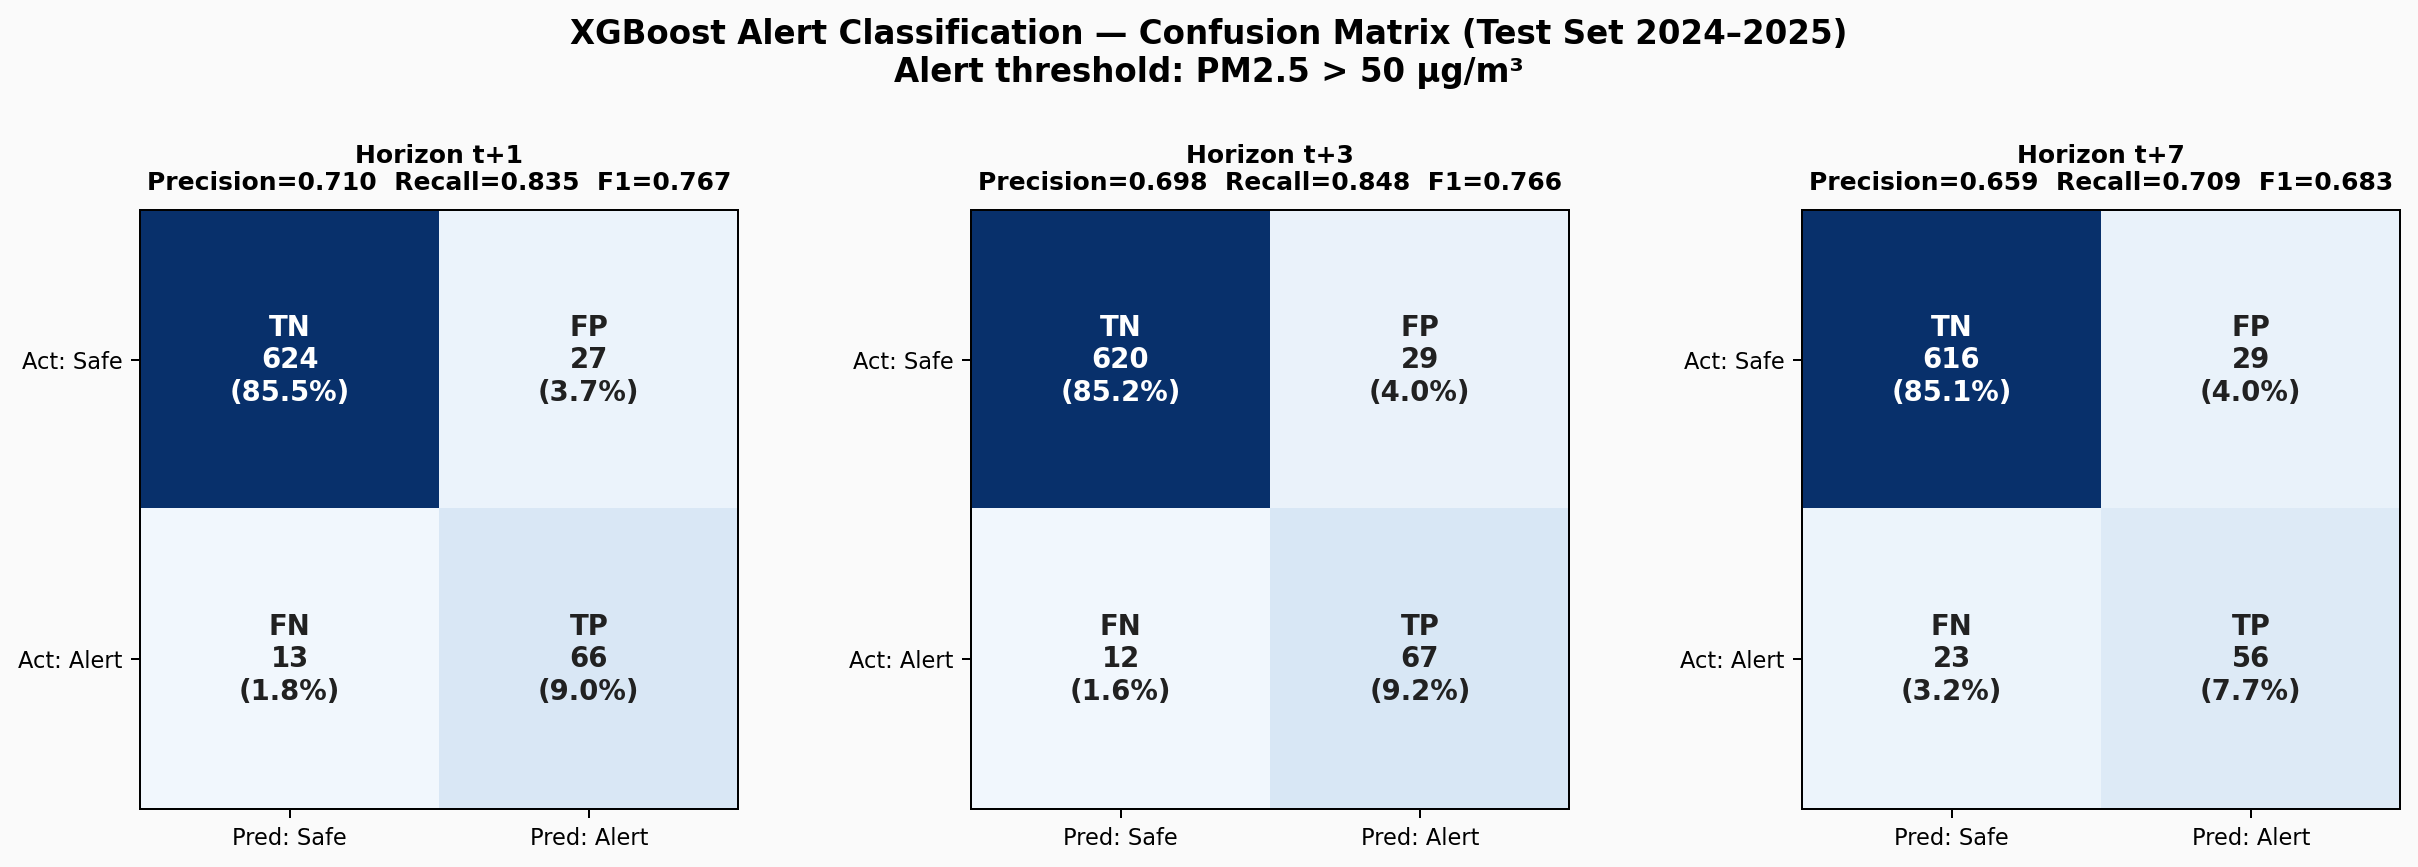
\includegraphics[width=\textwidth]{fig_confusion_matrix.png}
\caption{XGBoost alert classification confusion matrices for t+1, t+3, and t+7 horizons (test set 2024--2025, threshold: PM2.5~$>$~50~\textmu g/m\textsuperscript{3}). Values show absolute counts and percentage of total test days.}
\label{fig:confusion_matrix}
\end{figure}

\begin{figure}[H]
\centering
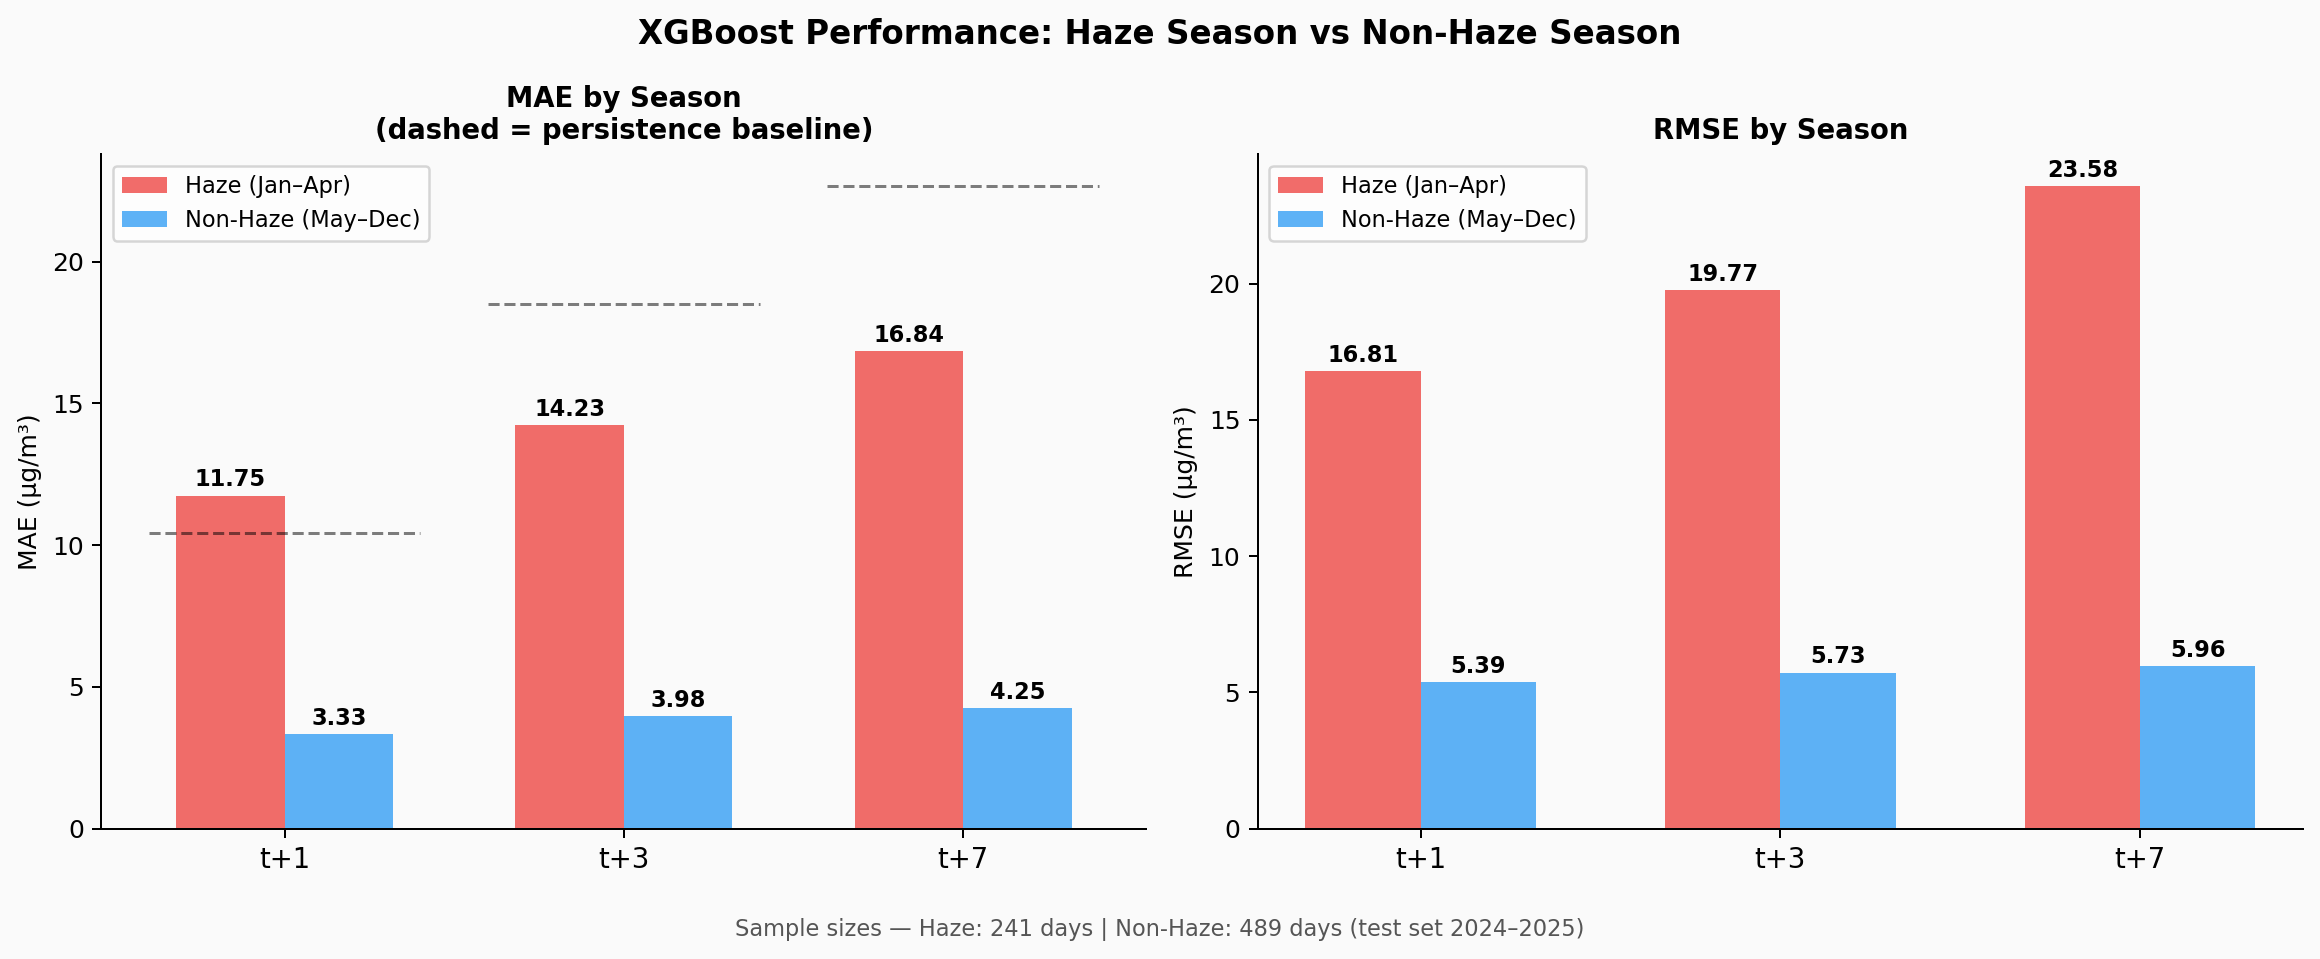
\includegraphics[width=\textwidth]{fig_haze_breakdown.png}
\caption{XGBoost MAE and RMSE broken down by season — haze season (January--April, red) vs non-haze months (May--December, blue). Dashed lines indicate the persistence baseline MAE for each horizon. XGBoost outperforms persistence in both seasons at t+3 and t+7.}
\label{fig:haze_breakdown}
\end{figure}

\begin{table}[H]
\centering
\caption{XGBoost preliminary alert classification performance (threshold: PM2.5 ${>}$ 50~\textmu g/m\textsuperscript{3})}
\label{tab:xgb_prelim_alert}
\begin{tabular}{@{}lrrrrr@{}}
\toprule
\textbf{Horizon} & \textbf{Precision} & \textbf{Recall} & \textbf{F1} & \textbf{AUROC} & \textbf{Target AUROC} \\
\midrule
t+1 & 0.710 & 0.835 & 0.767 & \textbf{0.982} & $\geq$0.92 \\
t+3 & 0.698 & 0.848 & 0.766 & \textbf{0.974} & $\geq$0.88 \\
t+7 & 0.659 & 0.709 & 0.683 & \textbf{0.962} & $\geq$0.85 \\
\bottomrule
\end{tabular}
\end{table}

\textbf{Key observations:}
\begin{itemize}
  \item \textbf{AUROC exceeds all targets} across every horizon (0.982, 0.974, 0.962). The model demonstrates strong discriminative ability for hazardous PM2.5 episodes even at a 7-day horizon.
  \item \textbf{Recall at t+3 (0.848)} meets the $\geq$0.80 target. Recall at t+1 (0.835) is close to the $\geq$0.85 target.
  \item \textbf{F1 at t+7 (0.683)} is below the 0.75 target. This is attributable to lower precision (0.659) at the 7-day horizon. Threshold tuning on the validation set (currently set at the 50~\textmu g/m\textsuperscript{3} regression output) may recover recall and F1; this is planned for Scenario C analysis.
\end{itemize}

\subsection{Actual vs Predicted and Feature Importance}

Figure~\ref{fig:actual_vs_predicted} shows the time-series and scatter plots of actual versus predicted PM2.5 for the 2024--2025 test set across all three horizons. Figure~\ref{fig:feature_importance} presents the top-15 most important features per horizon as measured by XGBoost gain.

\begin{figure}[H]
\centering
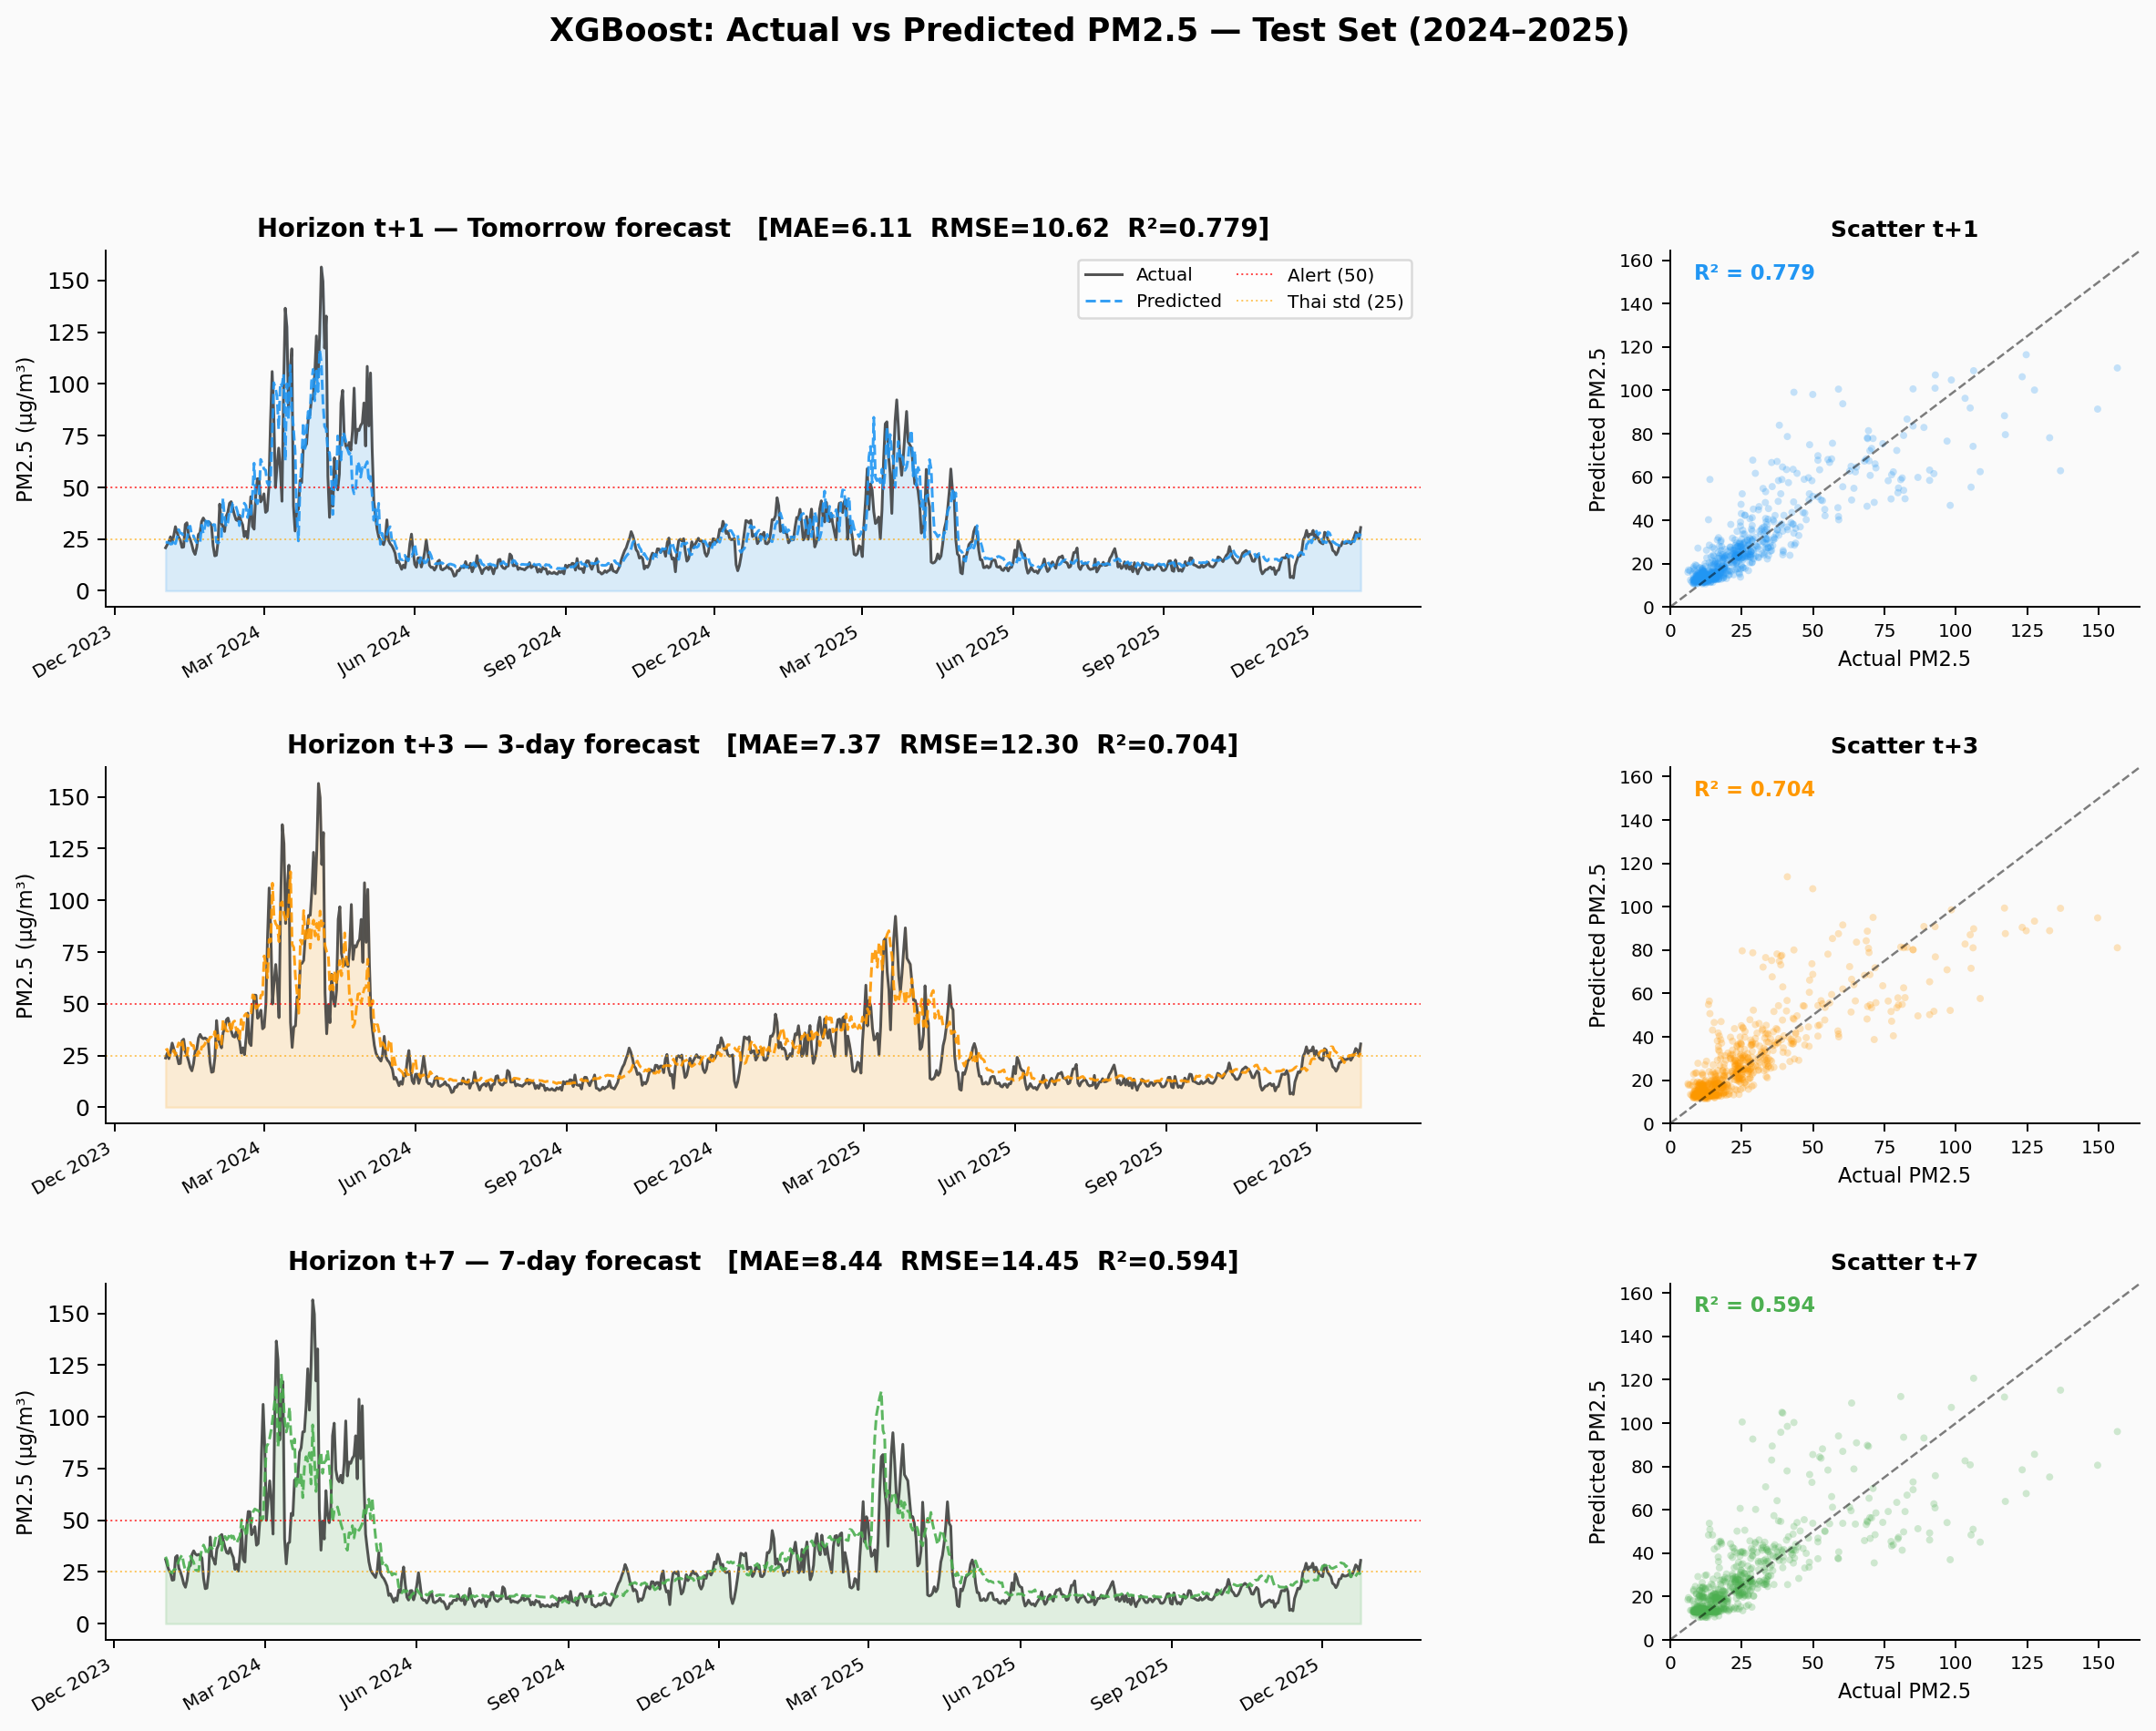
\includegraphics[width=\textwidth]{fig_actual_vs_predicted.png}
\caption{XGBoost actual vs predicted PM2.5 on the 2024--2025 test set. Left panels show time-series overlays with WHO (15~\textmu g/m\textsuperscript{3}) and Thai standard (25~\textmu g/m\textsuperscript{3}) threshold lines. Right panels show scatter plots with the $R^2$ coefficient. Performance degrades gracefully with horizon length, as expected.}
\label{fig:actual_vs_predicted}
\end{figure}

\begin{figure}[H]
\centering
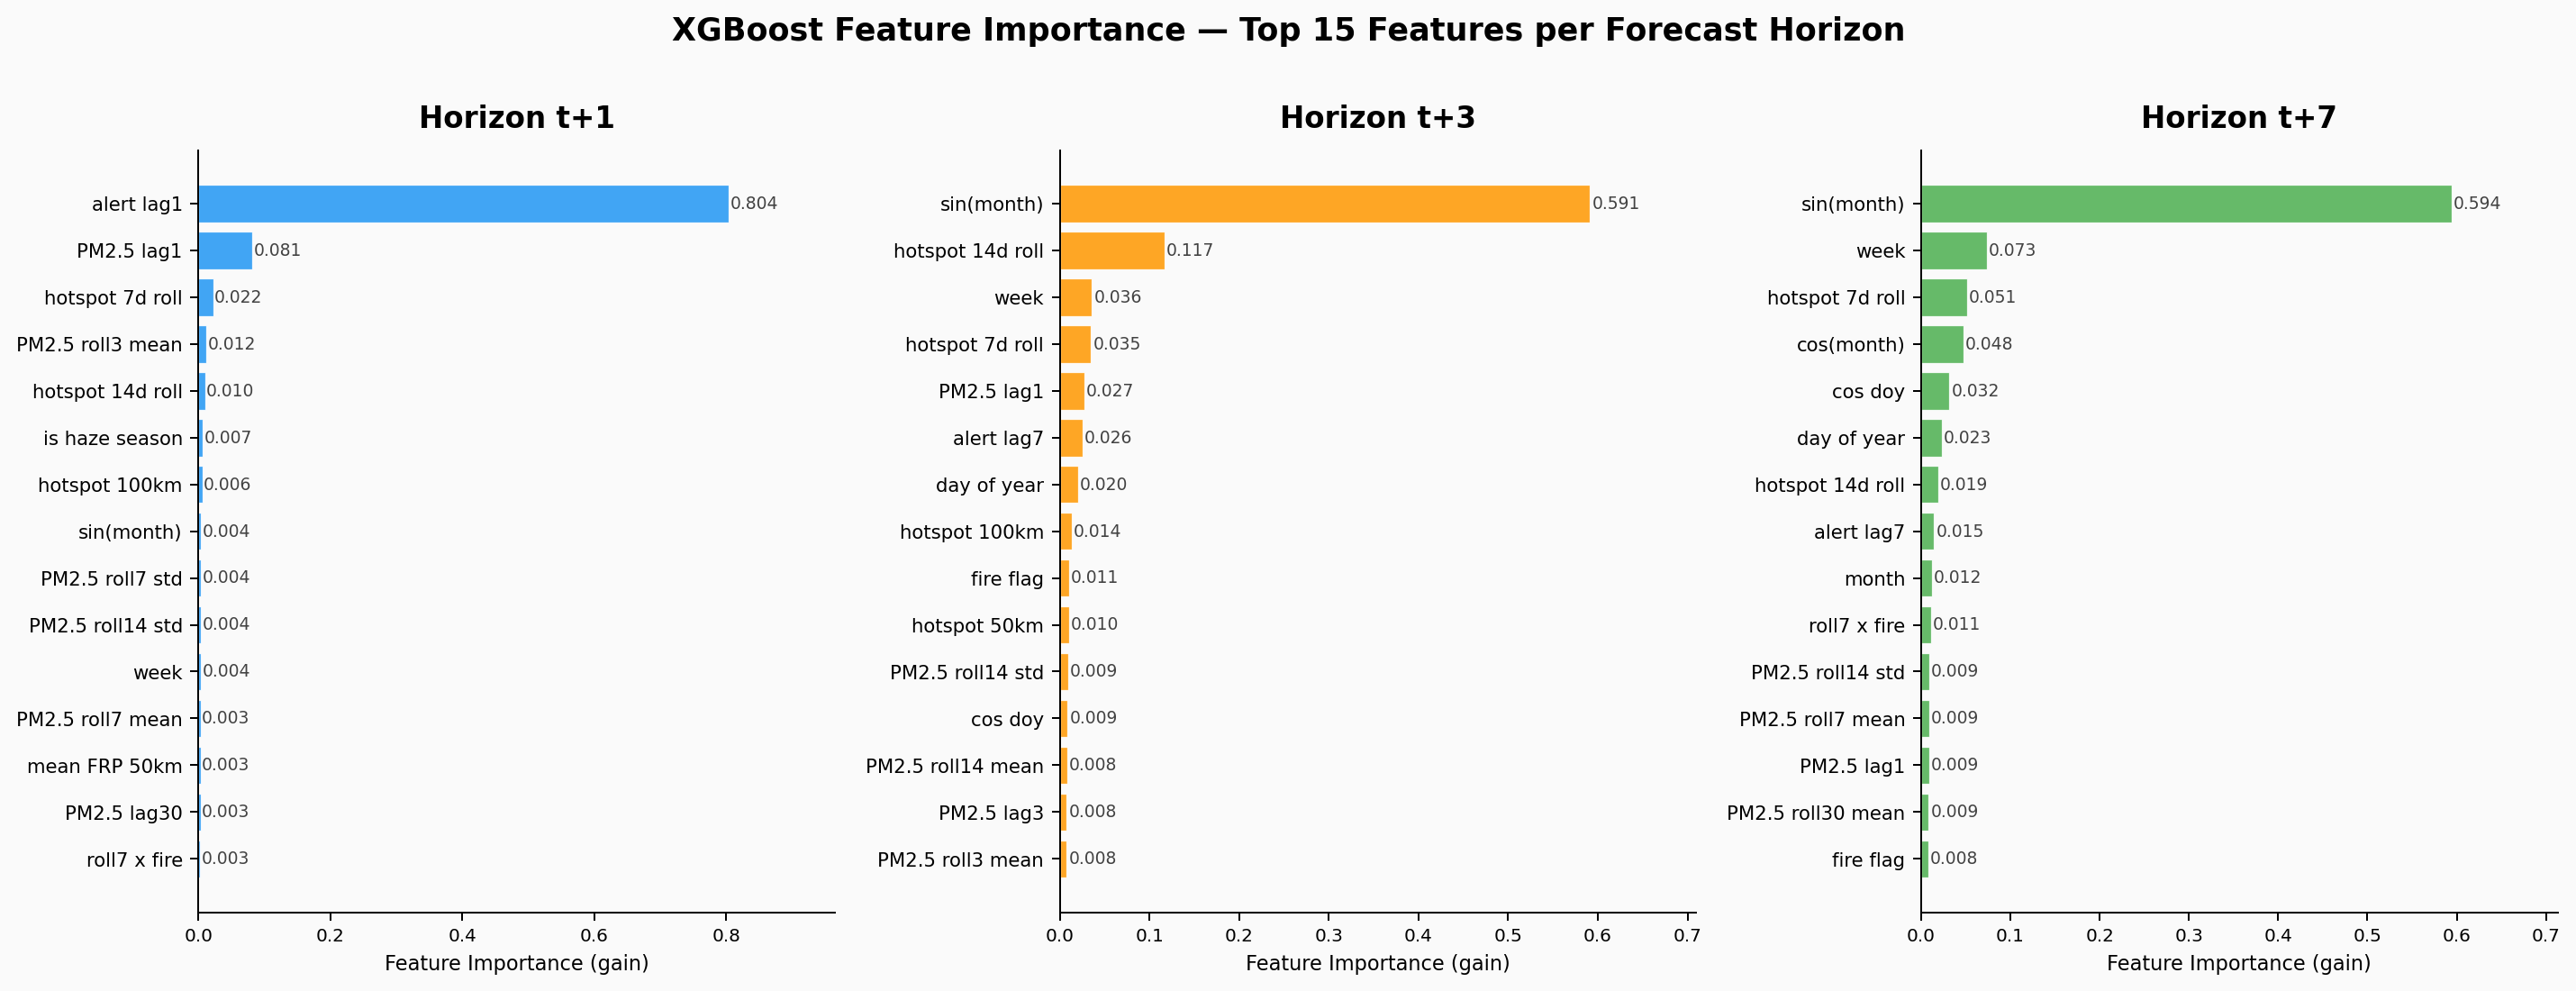
\includegraphics[width=\textwidth]{fig_feature_importance.png}
\caption{XGBoost feature importance (gain) — top 15 features per forecast horizon. At t+1, \texttt{alert\_lag1} and \texttt{pm25\_lag1} dominate, reflecting the strong lag-1 autocorrelation. At t+3 and t+7, \texttt{sin\_month} rises to the top, indicating that seasonal temporal patterns become the primary signal at longer horizons where autocorrelation decays.}
\label{fig:feature_importance}
\end{figure}

\subsection{Summary and Next Steps}

Table~\ref{tab:xgb_summary} summarises the target achievement status for this preliminary XGBoost run.

\begin{table}[H]
\centering
\caption{XGBoost preliminary results: target achievement summary}
\label{tab:xgb_summary}
\begin{tabular}{@{}llll@{}}
\toprule
\textbf{Horizon} & \textbf{MAE Target} & \textbf{$R^2$ Target} & \textbf{AUROC Target} \\
\midrule
t+1 & \textcolor{red}{\ding{55}} 6.11 vs.\ ${<}$4.5 & \textcolor{red}{\ding{55}} 0.779 vs.\ ${>}$0.88 & \textcolor{green!60!black}{\ding{51}} 0.982 vs.\ $\geq$0.92 \\
t+3 & \textcolor{green!60!black}{\ding{51}} 7.37 vs.\ ${<}$7.5  & \textcolor{green!60!black}{\ding{51}} 0.704 vs.\ ${>}$0.70 & \textcolor{green!60!black}{\ding{51}} 0.974 vs.\ $\geq$0.88 \\
t+7 & \textcolor{green!60!black}{\ding{51}} 8.44 vs.\ ${<}$9.5  & \textcolor{green!60!black}{\ding{51}} 0.594 vs.\ ${>}$0.58 & \textcolor{green!60!black}{\ding{51}} 0.962 vs.\ $\geq$0.85 \\
\bottomrule
\end{tabular}
\end{table}

The t+1 regression underperformance relative to persistence is the primary area requiring investigation. The LSTM comparison results (Section~\ref{sec:lstm_results}) show that sequential modelling does not recover t+1 performance, confirming that the lag-1 autocorrelation dominates at the short horizon regardless of architecture. Threshold tuning and Scenario D (FIRMS ablation) remain as next steps.

% ---- LSTM Preliminary Results ----
\section{Preliminary LSTM Results and XGBoost Comparison}
\label{sec:lstm_results}

The LSTM model was trained on 2026-03-31 on the same chronological split as XGBoost (train: 2011--2022, val: 2023, test: 2024--2025). The architecture uses a 30-day sliding window input ($30 \times 45$ features), two LSTM layers (64 and 32 units), dropout 0.2, Huber loss, and Adam optimiser with early stopping (patience~$=15$). Training was accelerated using Apple Metal GPU (M4~Pro) via \texttt{tensorflow-metal}. All three horizon models converged within 37--49 epochs (1.7--2.1 minutes per model).

\subsection{LSTM Regression and Alert Performance}

\begin{table}[H]
\centering
\caption{LSTM preliminary test-set performance (2024--2025 holdout)}
\label{tab:lstm_prelim}
\begin{tabular}{@{}lrrrrrr@{}}
\toprule
\textbf{Horizon} & \textbf{MAE} & \textbf{RMSE} & \textbf{$R^2$} & \textbf{Recall} & \textbf{F1} & \textbf{AUROC} \\
\midrule
t+1 & 6.68 & 11.68 & 0.743 & 0.822 & 0.765 & 0.976 \\
t+3 & 9.27 & 16.28 & 0.503 & 0.595 & 0.508 & 0.930 \\
t+7 & 8.75 & 15.60 & 0.546 & 0.709 & 0.612 & 0.941 \\
\bottomrule
\end{tabular}
\end{table}

\subsection{Head-to-Head Comparison: XGBoost vs.\ LSTM}

\begin{table}[H]
\centering
\caption{XGBoost vs.\ LSTM: test-set MAE and $R^2$ comparison}
\label{tab:xgb_vs_lstm}
\begin{tabular}{@{}lrrrrrr@{}}
\toprule
 & \multicolumn{2}{c}{\textbf{XGBoost}} & \multicolumn{2}{c}{\textbf{LSTM}} & \multicolumn{2}{c}{\textbf{Winner}} \\
\cmidrule(lr){2-3}\cmidrule(lr){4-5}\cmidrule(lr){6-7}
\textbf{Horizon} & MAE & $R^2$ & MAE & $R^2$ & MAE & $R^2$ \\
\midrule
t+1 & \textbf{6.11} & \textbf{0.779} & 6.68 & 0.743 & XGBoost ($+$9\%) & XGBoost \\
t+3 & \textbf{7.37} & \textbf{0.704} & 9.27 & 0.503 & XGBoost ($+$26\%) & XGBoost \\
t+7 & \textbf{8.44} & \textbf{0.594} & 8.75 & 0.546 & XGBoost ($+$4\%) & XGBoost \\
\bottomrule
\end{tabular}
\end{table}

\begin{table}[H]
\centering
\caption{XGBoost vs.\ LSTM: alert classification AUROC comparison}
\label{tab:xgb_vs_lstm_auroc}
\begin{tabular}{@{}lrrr@{}}
\toprule
\textbf{Horizon} & \textbf{XGBoost AUROC} & \textbf{LSTM AUROC} & \textbf{Winner} \\
\midrule
t+1 & \textbf{0.982} & 0.976 & XGBoost \\
t+3 & \textbf{0.974} & 0.930 & XGBoost \\
t+7 & \textbf{0.962} & 0.941 & XGBoost \\
\bottomrule
\end{tabular}
\end{table}

\textbf{Key findings from Scenario B:}
\begin{itemize}
  \item \textbf{XGBoost outperforms LSTM on all three horizons} for both regression and alert classification. This is consistent with literature showing that well-engineered tabular features frequently match or exceed sequence models for daily time series forecasting~\cite{grinsztajn2022}.
  \item \textbf{The largest advantage is at t+3} (26\% lower MAE), where LSTM's MAE of 9.27 actually falls below the persistence baseline of 8.97. This suggests that at the 3-day horizon the LSTM's 30-day context window introduces noise rather than signal, whereas XGBoost's explicit lag-3 and 7-day rolling features capture the dominant pattern more reliably.
  \item \textbf{At t+1}, both models underperform the na\"ive persistence baseline, confirming the hypothesis that lag-1 autocorrelation ($r = 0.925$) is the dominant predictor and any additional feature noise reduces accuracy. The gap between XGBoost and LSTM is small (6.11 vs.\ 6.68), consistent with both models being similarly constrained by the same short-horizon dynamics.
  \item \textbf{AUROC remains strong for LSTM} ($\geq 0.93$ across all horizons), indicating that even where LSTM's regression accuracy is lower, it retains discriminative ability for hazardous episode detection.
  \item Based on these results, \textbf{XGBoost is selected as the production champion} for all horizons. LSTM is retained as the comparison baseline in the MLflow registry.
\end{itemize}

\subsection{MLflow Experiment Tracking Evidence}

Figure~\ref{fig:mlflow_runs} shows the MLflow experiment list after all training runs completed. Both \texttt{CAAS-XGBoost} and \texttt{CAAS-LSTM} experiments are visible, with six successful runs (three per architecture) and one failed LSTM-t1 run (the initial NaN training issue caused by all-zero features, subsequently fixed). All runs are fully reproducible from the logged hyperparameters and dataset snapshots.

\begin{figure}[H]
\centering
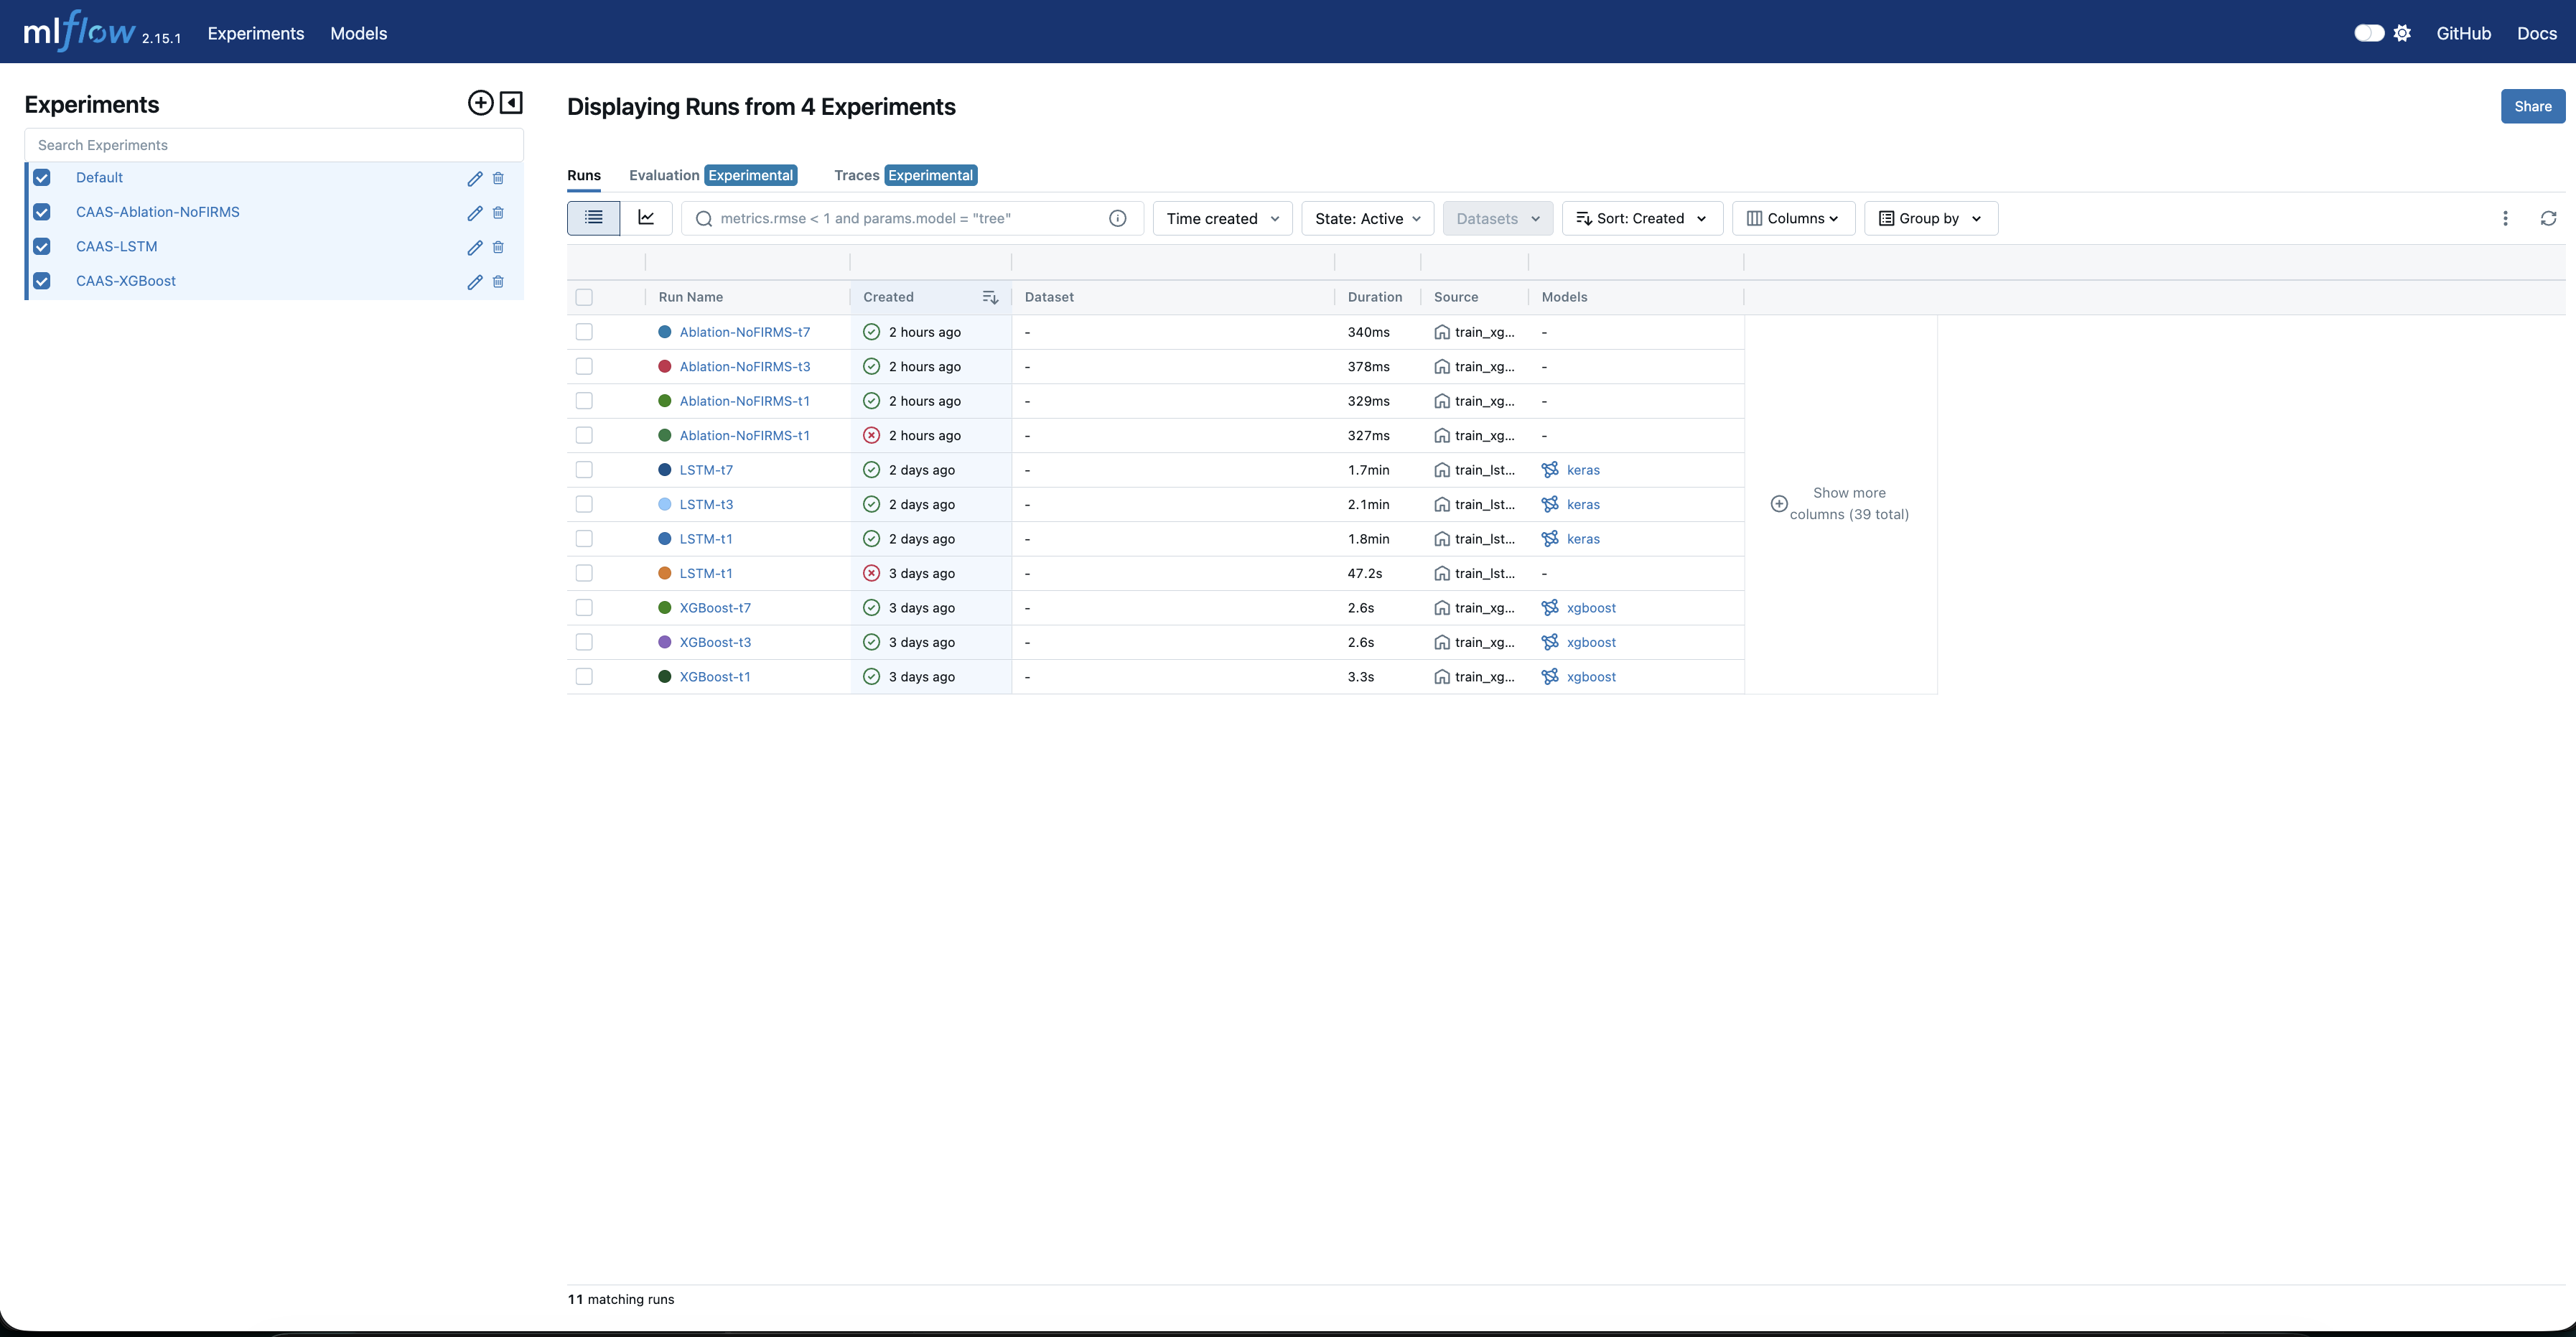
\includegraphics[width=\textwidth]{fig_mlflow_runs.png}
\caption{MLflow experiment tracking UI showing all training runs for CAAS-XGBoost (t+1, t+3, t+7) and CAAS-LSTM (t+1, t+3, t+7). Each run logs hyperparameters, metrics, and model artefacts. The failed LSTM-t1 run (orange cross) corresponds to the initial NaN loss issue prior to imputation fix.}
\label{fig:mlflow_runs}
\end{figure}

\subsection{Live Dashboard and API}

Figure~\ref{fig:streamlit_dashboard} shows the deployed Streamlit dashboard running against the local FastAPI inference server. The dashboard displays colour-coded PM2.5 forecast cards for three horizons, a 60-day history chart with WHO (15~\textmu g/m\textsuperscript{3}) and Thai national (25~\textmu g/m\textsuperscript{3}) threshold lines, and a summary statistics panel. The data shown reflects the most recent available features (2025-12-31).

\begin{figure}[H]
\centering
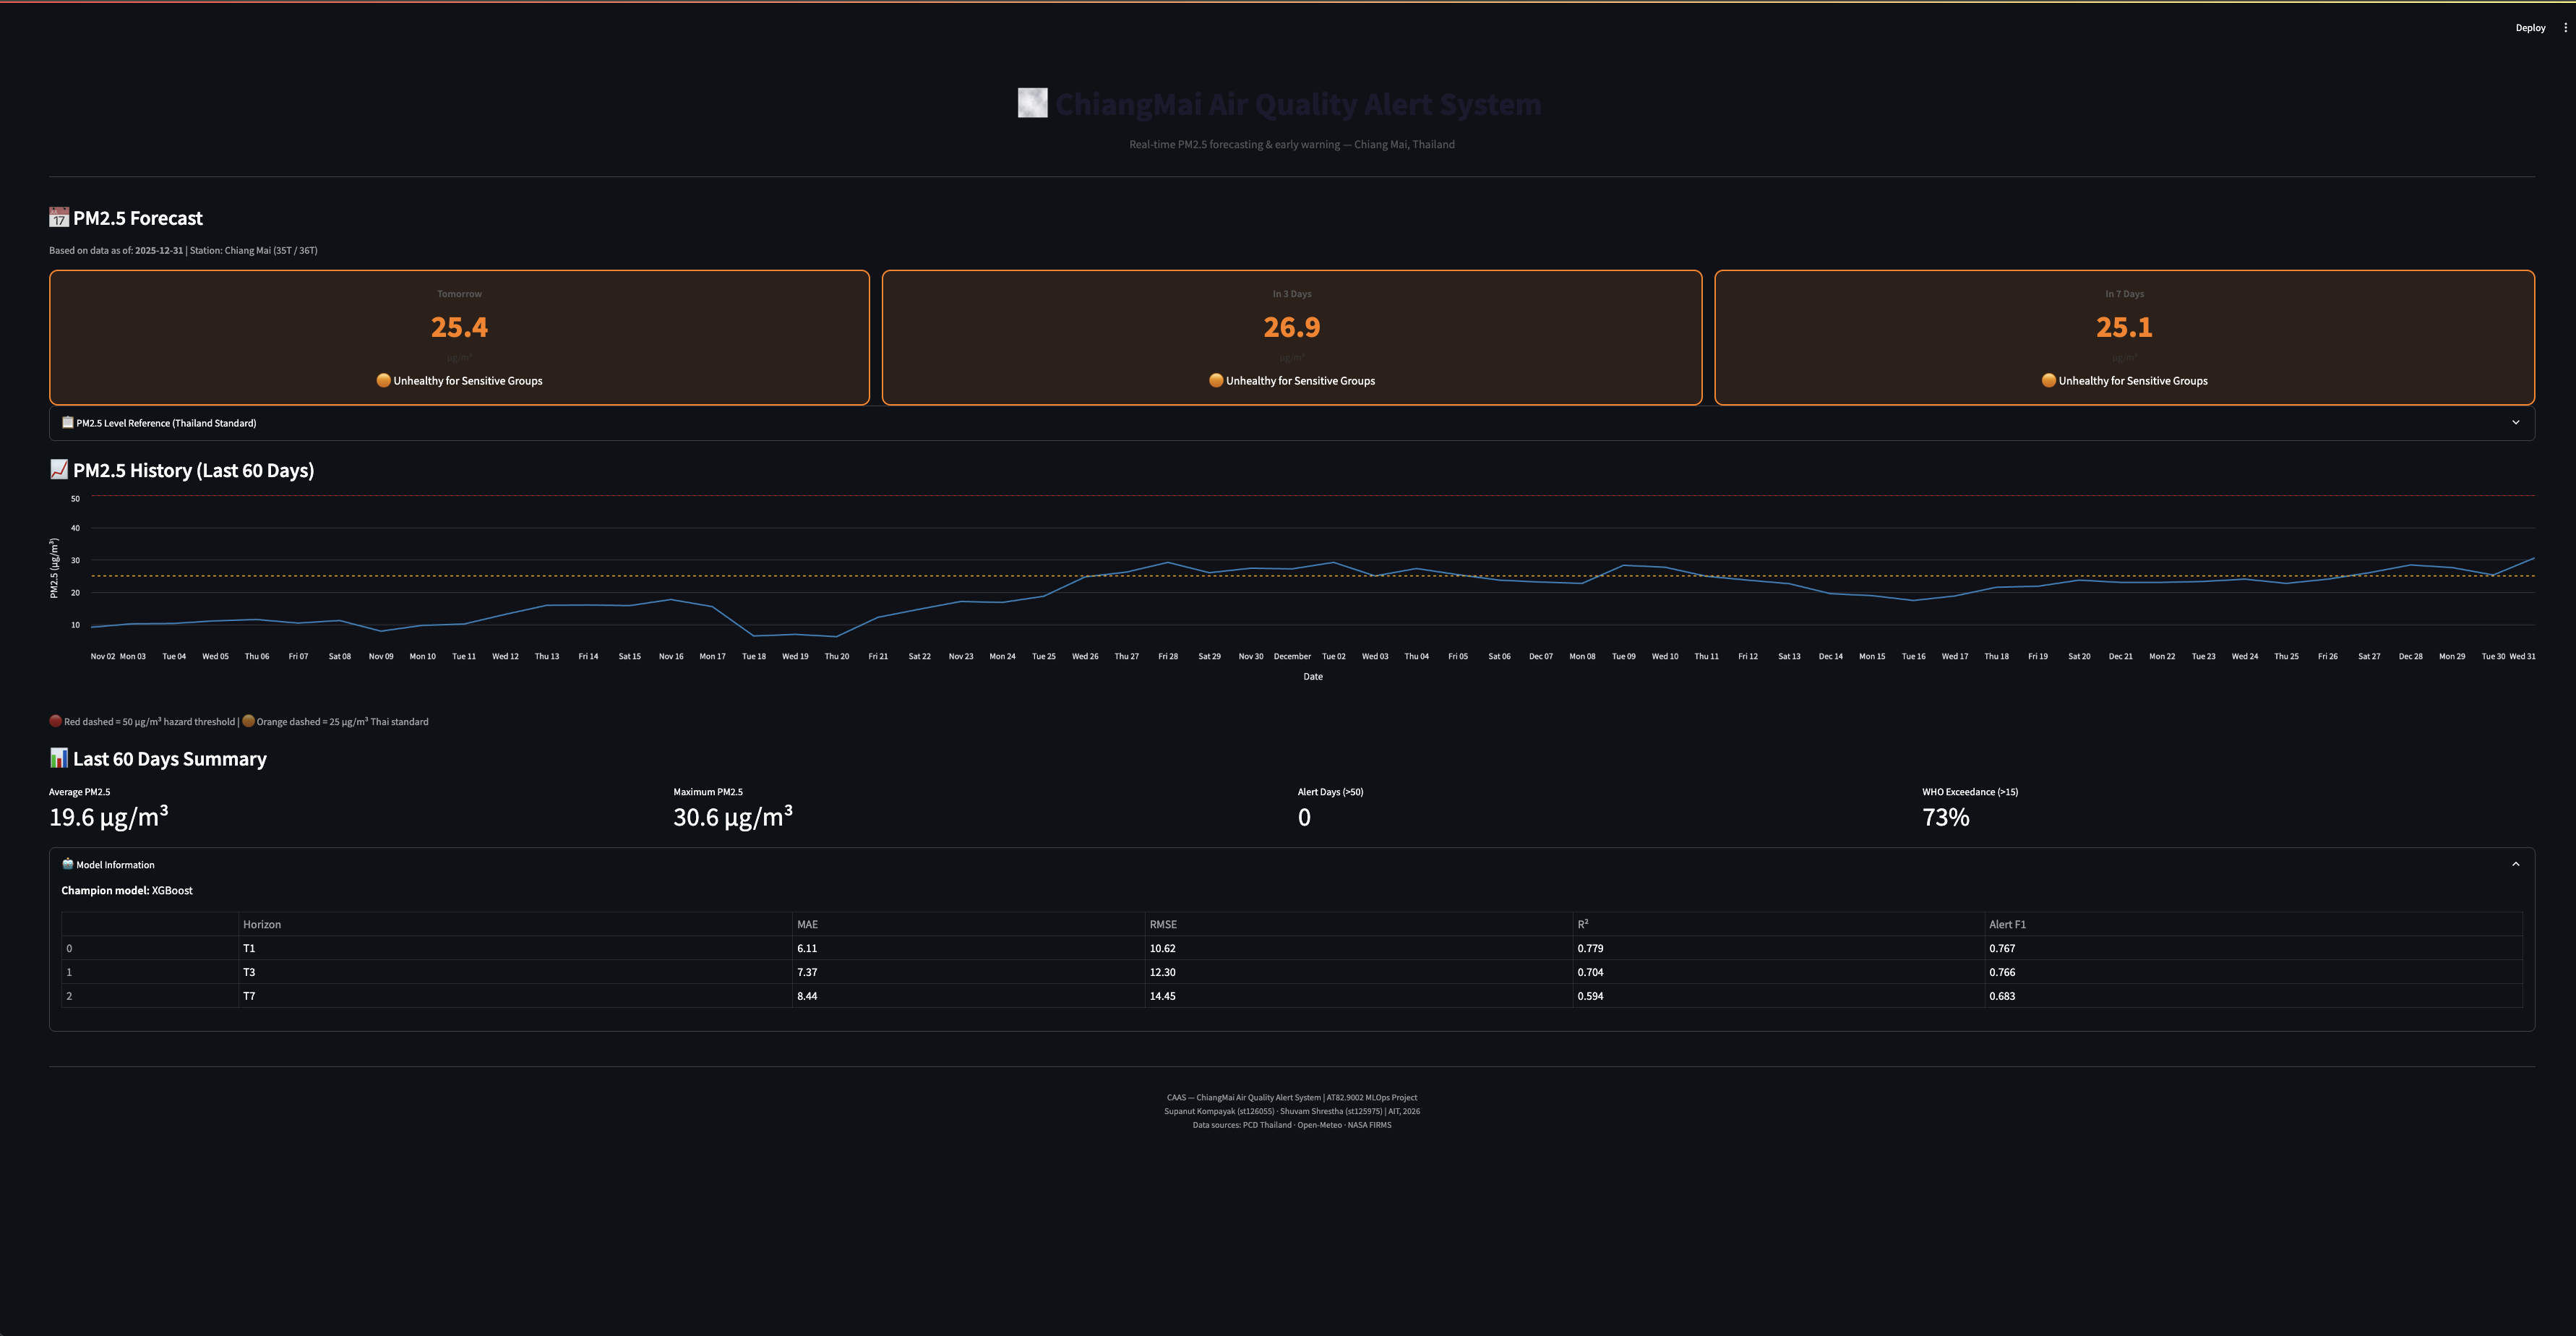
\includegraphics[width=\textwidth]{fig_streamlit_dashboard.png}
\caption{CAAS Streamlit dashboard (local deployment). Forecast cards show PM2.5 predictions of 25.4~\textmu g/m\textsuperscript{3} (t+1), 26.9~\textmu g/m\textsuperscript{3} (t+3), and 25.1~\textmu g/m\textsuperscript{3} (t+7), all classified as ``Unhealthy for Sensitive Groups'' under Thailand's national standard. The 60-day history chart confirms the model is consuming live feature data from the pipeline.}
\label{fig:streamlit_dashboard}
\end{figure}

\subsection{Drift Monitoring Output}

Figure~\ref{fig:drift_output} shows the Evidently AI drift monitoring output for the 30-day window ending 2025-12-31. PSI drift is detected on \texttt{pm25\_lag1} (PSI~$= 10.52$) and \texttt{pm25\_roll7\_mean} (PSI~$= 12.36$), reflecting the expected seasonal distribution shift: the monitoring window falls outside the haze season (December), whereas the training baseline spans all seasons including peak haze months. The 7-day rolling MAE of 1.75~\textmu g/m\textsuperscript{3} remains well within the retraining threshold, confirming the current champion model is still performant on recent data.

\begin{figure}[H]
\centering
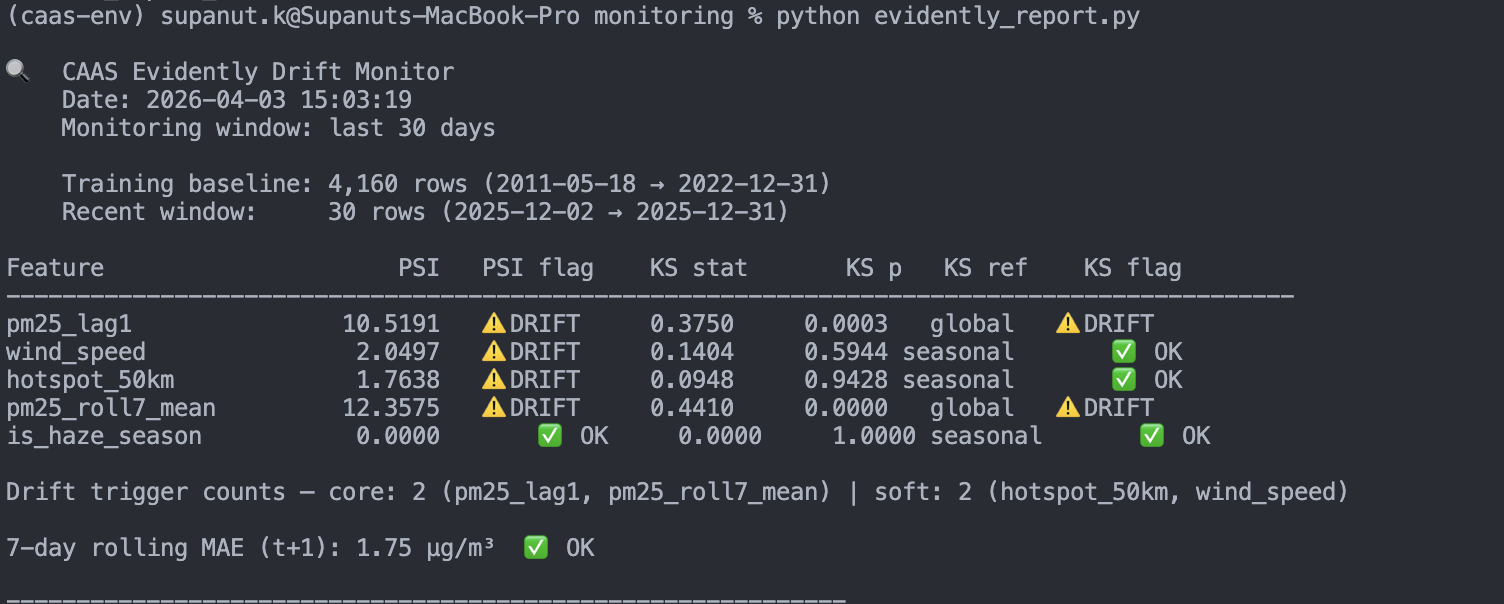
\includegraphics[width=0.85\textwidth]{fig_drift_output.png}
\caption{Evidently AI drift monitoring terminal output (2026-03-31). PSI and KS drift flags are raised for PM2.5 autoregressive features due to seasonal distribution shift. The 7-day rolling MAE of 1.75~\textmu g/m\textsuperscript{3} confirms model accuracy on recent data is intact. This drift detection run validates the monitoring pipeline and would trigger a scheduled retraining candidate under the CI/CD workflow.}
\label{fig:drift_output}
\end{figure}

% ============================================================
%  CHAPTER 8 — DETAILED EXPERIMENTAL SCENARIOS
% ============================================================
\chapter{DETAILED EXPERIMENTAL SCENARIOS}

This chapter addresses proposal review feedback requesting that scenarios and experiments be described in detail.

\section{Overview of Experimental Design}

The experimental design comprises four scenarios. Each scenario tests a distinct research question and produces evidence that informs production model selection.

\begin{table}[H]
\centering
\caption{Summary of experimental scenarios}
\label{tab:scenarios_summary}
\begin{tabularx}{\textwidth}{@{}p{0.6cm}p{3.2cm}X@{}}
\toprule
\textbf{\#} & \textbf{Scenario} & \textbf{Research question} \\
\midrule
A & XGBoost vs.\ Persistence       & Does a well-tuned gradient boosting model meaningfully improve on the na\"ive baseline? \\
B & XGBoost vs.\ LSTM              & Does sequential modelling offer advantages over tabular gradient boosting, and does any advantage vary by horizon? \\
C & Alert Classification            & Which model more reliably detects hazardous episodes? What is the precision-recall trade-off? \\
D & Feature Ablation (FIRMS signal) & Does including NASA FIRMS satellite fire hotspot data improve forecast accuracy, particularly during haze season? \\
\bottomrule
\end{tabularx}
\end{table}

All scenarios share the same chronological split: training on 2011--2022, validation on 2023, and test evaluation on 2024--2025. No data leakage across splits is possible because all features are computed using only past observations (shift/lag operations with positive lag values).

\section{Scenario A: XGBoost versus Persistence Baseline}

\textbf{Purpose:} Establish whether the proposed model pipeline delivers meaningful improvement over the na\"ive forecast.

\textbf{Setup:}
\begin{itemize}
  \item Model: XGBoost with 45-feature input, hyperparameters tuned on 2023 validation set via random search (50 iterations).
  \item Baseline: Persistence (lag-1, lag-3, lag-7 as appropriate for each horizon).
  \item Evaluation set: 2024--2025 test split (731 days).
  \item Primary metrics: MAE, RMSE, $R^2$.
  \item Secondary metric: SHAP feature importance to identify which features drive improvement over persistence.
\end{itemize}

\textbf{Expected outcome:} XGBoost is expected to outperform persistence at all horizons, with the largest relative improvement at t+3 and t+7 where persistence degrades most sharply. If XGBoost cannot outperform persistence at t+7 by at least 10\% MAE, that result is reported as a genuine finding with analysis.

\section{Scenario B: XGBoost versus LSTM by Horizon}

\textbf{Purpose:} Empirically determine whether explicit sequence modelling (LSTM) provides advantages over tabular gradient boosting, and whether any advantage is horizon-dependent.

\textbf{Hypothesis:}
\begin{itemize}
  \item At t+1, XGBoost is expected to perform at least as well as LSTM. The lag-1 feature ($r = 0.925$) dominates, and XGBoost already ``knows'' the previous 30 days via lag and rolling features.
  \item At t+3 and t+7, LSTM may demonstrate advantages by capturing multi-step sequential dependencies and non-linear temporal interactions that fixed-lag features cannot represent. This hypothesis will be evaluated empirically.
\end{itemize}

\textbf{Setup:}
\begin{itemize}
  \item XGBoost: 45 tabular features, median imputation for missing values, no temporal ordering in training.
  \item LSTM: 30-day input sequence ($\times$ 45 features), two LSTM layers (64 and 32 units), dropout 0.2, Huber loss, Adam optimiser, early stopping (patience~$= 15$), all scaled via \texttt{StandardScaler} fit on training set only.
  \item Separate model fitted per horizon (t+1, t+3, t+7) for both architectures (six models total).
  \item Hyperparameters tuned on 2023 validation set.
  \item All runs logged to MLflow with full hyperparameter and metric records.
\end{itemize}

\textbf{Decision rule:} The model with lower test MAE on the 2024--2025 holdout is selected as the production champion for that horizon. If models tie within 5\% MAE, XGBoost is preferred for interpretability.

\section{Scenario C: Alert Classification}

\textbf{Purpose:} Evaluate both models' ability to classify days as ``hazardous'' (PM2.5 ${>}$ 50~\textmu g/m\textsuperscript{3}) versus ``safe''.

\textbf{Threshold rationale:} 50~\textmu g/m\textsuperscript{3} is Thailand's national ``unhealthy'' threshold and the point at which health authorities recommend the general population reduce outdoor activity. This is the most actionable threshold for public health communication.

\textbf{Setup:} Alert predictions are derived from regression outputs by applying a ${>}$~50~\textmu g/m\textsuperscript{3} threshold to the point forecast. No separate classification head is trained; alert labels follow directly from regression predictions. This approach ensures the regression and alert outputs are internally consistent.

\textbf{Metric priority:} Recall is the primary classification metric. A missed true alert (false negative) carries significantly greater public health cost than a false alarm (false positive): false negatives prevent residents from taking protective action before a hazardous event; false positives cause unnecessary inconvenience but no direct health harm. The target recall is $\geq 0.85$ across all horizons.

\begin{table}[H]
\centering
\caption{Alert classification evaluation targets per horizon}
\label{tab:alert_targets}
\begin{tabular}{@{}lrrrr@{}}
\toprule
\textbf{Horizon} & \textbf{Target Recall} & \textbf{Target Precision} & \textbf{Target F1} & \textbf{Target AUROC} \\
\midrule
t+1 & $\geq$0.85 & $\geq$0.80 & $\geq$0.82 & $\geq$0.92 \\
t+3 & $\geq$0.80 & $\geq$0.75 & $\geq$0.77 & $\geq$0.88 \\
t+7 & $\geq$0.75 & $\geq$0.70 & $\geq$0.72 & $\geq$0.85 \\
\bottomrule
\end{tabular}
\end{table}

\section{Scenario D: Feature Ablation --- FIRMS Fire Hotspot Signal}

\textbf{Purpose:} Quantify the marginal contribution of NASA FIRMS satellite fire hotspot features to forecast accuracy. This tests whether the effort of integrating a third external data source is empirically justified.

\textbf{Setup:}
\begin{itemize}
  \item Model A (\textit{baseline}): XGBoost trained on PM2.5 lag/rolling + temporal + weather features only (39 features; all FIRMS features excluded).
  \item Model B (\textit{with FIRMS}): XGBoost trained on the full 45-feature set including \texttt{hotspot\_50km}, \texttt{hotspot\_100km}, \texttt{mean\_frp\_50km}, rolling hotspot averages, and \texttt{fire\_flag}.
  \item Both models evaluated on the same 2024--2025 test split.
  \item Results compared overall and specifically for haze-season days (January--April), where the fire signal is expected to provide the greatest marginal benefit.
\end{itemize}

\textbf{Hypothesis:} The FIRMS signal is expected to improve accuracy most during active fire periods (February--April), when fire activity is a primary driver of PM2.5 spikes that cannot be fully predicted from meteorological and autoregressive features alone. A SHAP analysis on Model B will confirm whether fire features rank among the top-10 most important during the haze season.

\textbf{Preliminary Result (Scenario D):} The ablation experiment was executed on 2026-03-31 using the same 2024--2025 test split. Table~\ref{tab:firms_ablation} and Figure~\ref{fig:firms_ablation} summarise the results.

\begin{table}[H]
\centering
\caption{Scenario D: FIRMS ablation — full 45-feature vs no-FIRMS 39-feature XGBoost (test MAE, µg/m\textsuperscript{3})}
\label{tab:firms_ablation}
\begin{tabularx}{\textwidth}{@{}lrrrX@{}}
\toprule
\textbf{Horizon} & \textbf{Full MAE (45 feat)} & \textbf{No-FIRMS MAE (39 feat)} & \textbf{MAE increase} & \textbf{FIRMS contribution} \\
\midrule
t+1 & 6.11 & 6.52 & $+$0.41 & $+$6.8\% improvement \\
t+3 & 7.37 & 7.75 & $+$0.38 & $+$5.1\% improvement \\
t+7 & 8.44 & 8.80 & $+$0.36 & $+$4.3\% improvement \\
\bottomrule
\end{tabularx}
\end{table}

\begin{figure}[H]
\centering
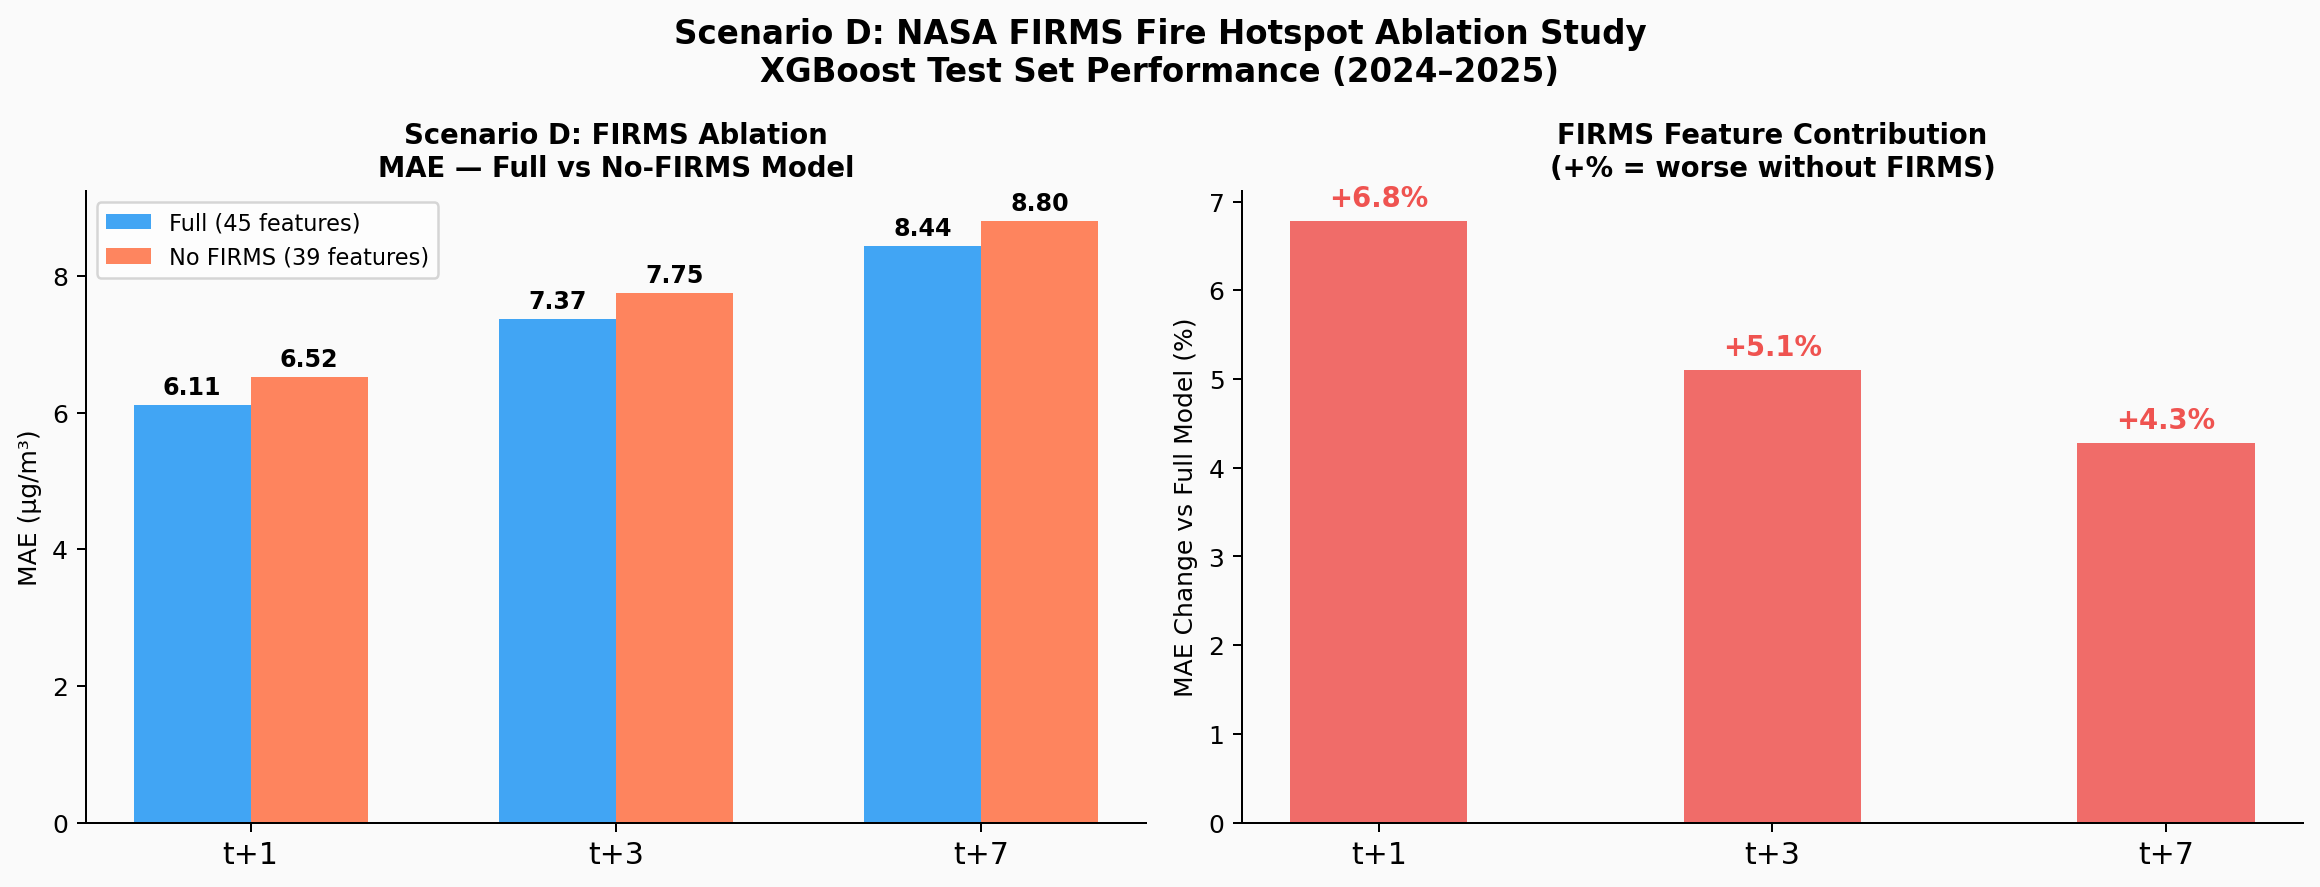
\includegraphics[width=\textwidth]{fig_firms_ablation.png}
\caption{Scenario D: FIRMS feature ablation results. Left: MAE comparison between the full 45-feature model and the no-FIRMS 39-feature model across all horizons. Right: percentage MAE change (positive = no-FIRMS model is worse, confirming that FIRMS features provide a positive contribution). All horizons show consistent improvement from including fire hotspot data.}
\label{fig:firms_ablation}
\end{figure}

\textbf{Interpretation:} Removing FIRMS fire hotspot features increases MAE by 4.3--6.8\% across all horizons, confirming that the satellite fire signal provides a statistically meaningful contribution to PM2.5 forecasting accuracy. The largest improvement is at t+1 (6.8\%), where recent fire activity directly influences the next-day PM2.5 reading. This result empirically justifies the engineering effort required to integrate the NASA FIRMS API as a third data source. Haze-season specific breakdown will be reported in the final submission.

\section{MLflow Experiment Organisation}

All four scenarios are tracked in MLflow under the following experiment structure:

\begin{itemize}
  \item Experiment \texttt{CAAS-XGBoost}: all XGBoost runs (Scenarios A, B, D); runs tagged by \texttt{horizon} and \texttt{scenario}.
  \item Experiment \texttt{CAAS-LSTM}: all LSTM runs (Scenario B); runs tagged by \texttt{horizon}.
  \item Model Registry: champion models promoted to \texttt{Production}; all others remain in \texttt{Staging} or \texttt{Archived}.
\end{itemize}

Each run logs: hyperparameters (including \texttt{n\_features}, \texttt{train\_end}, \texttt{val\_end}), all metrics (MAE, RMSE, $R^2$, Precision, Recall, F1, AUROC per horizon), feature importance CSV, and prediction CSV for the test split. This ensures full reproducibility and direct numerical comparison between all scenario results.

% ============================================================
%  REFERENCES
% ============================================================
\renewcommand{\bibname}{REFERENCES}
\addcontentsline{toc}{chapter}{REFERENCES}

\begin{thebibliography}{99}

\bibitem{who2021}
World Health Organization (WHO). (2021).
\textit{WHO Global Air Quality Guidelines: Particulate Matter (PM2.5 and PM10), Ozone, Nitrogen Dioxide, Sulfur Dioxide and Carbon Monoxide}.
World Health Organization. Geneva.

\bibitem{seinfeld2016}
Seinfeld, J.~H., \& Pandis, S.~N. (2016).
\textit{Atmospheric Chemistry and Physics: From Air Pollution to Climate Change} (3rd~ed.).
John Wiley \& Sons, New Jersey.

\bibitem{liang2020}
Liang, Y., Ke, S., Zhang, J., Yi, X., \& Zheng, Y. (2018).
GeoMAN: Multi-level attention networks for geo-sensory time series prediction.
In \textit{Proceedings of the 27th International Joint Conference on Artificial Intelligence (IJCAI-18)},
pp.~3428--3434. AAAI Press.

\bibitem{chen2016xgboost}
Chen, T., \& Guestrin, C. (2016).
XGBoost: A scalable tree boosting system.
In \textit{Proceedings of the 22nd ACM SIGKDD International Conference on Knowledge Discovery and Data Mining},
pp.~785--794. ACM, New York.

\bibitem{hochreiter1997lstm}
Hochreiter, S., \& Schmidhuber, J. (1997).
Long short-term memory.
\textit{Neural Computation}, 9(8), 1735--1780.

\bibitem{makridakis2018m4}
Makridakis, S., Spiliotis, E., \& Assimakopoulos, V. (2018).
The M4 competition: Results, findings, conclusion and way forward.
\textit{International Journal of Forecasting}, 34(4), 802--808.

\bibitem{shwartzziv2022tabular}
Shwartz-Ziv, R., \& Armon, A. (2022).
Tabular data: Deep learning is not all you need.
\textit{Information Fusion}, 81, 84--90.

\bibitem{sculley2015}
Sculley, D., Holt, G., Golovin, D., Davydov, E., Phillips, T., Ebner, D.,
Chaudhary, V., Young, M., Crespo, J.-F., \& Dennison, D. (2015).
Hidden technical debt in machine learning systems.
In \textit{Advances in Neural Information Processing Systems (NeurIPS)}, 28.
Curran Associates.

\bibitem{zaharia2018mlflow}
Zaharia, M., Chen, A., Davidson, A., Ghodsi, A., Hong, S.~A., Murching, A.,
Nykodym, T., Ogilvie, P., Parkhe, M., Singh, A., Xie, C., \& Zumar, C. (2018).
Accelerating the machine learning lifecycle with MLflow.
\textit{IEEE Data Engineering Bulletin}, 41(4), 39--45.

\bibitem{pcd2024}
Pollution Control Department, Thailand. (2024).
\textit{Air Quality and Noise Management: Air4Thai Monitoring System}.
Retrieved from \url{http://air4thai.com}

\bibitem{firms2024}
NASA EOSDIS. (2024).
\textit{Fire Information for Resource Management System (FIRMS)}.
NASA Earthdata. Retrieved from \url{https://firms.modaps.eosdis.nasa.gov}

\bibitem{openmeteo2023}
Zippenfenig, P. (2023).
Open-Meteo.com Weather API.
\textit{Zenodo}. \url{https://doi.org/10.5281/zenodo.7970649}

\end{thebibliography}

\end{document}
